
\documentclass{article} % For LaTeX2e
\usepackage[svgnames]{xcolor}
\usepackage{iclr2024_conference,times}

% Optional math commands from https://github.com/goodfeli/dlbook_notation.
%%%%% NEW MATH DEFINITIONS %%%%%

\usepackage{amsmath,amsfonts,bm}

% Mark sections of captions for referring to divisions of figures
\newcommand{\figleft}{{\em (Left)}}
\newcommand{\figcenter}{{\em (Center)}}
\newcommand{\figright}{{\em (Right)}}
\newcommand{\figtop}{{\em (Top)}}
\newcommand{\figbottom}{{\em (Bottom)}}
\newcommand{\captiona}{{\em (a)}}
\newcommand{\captionb}{{\em (b)}}
\newcommand{\captionc}{{\em (c)}}
\newcommand{\captiond}{{\em (d)}}

% Highlight a newly defined term
\newcommand{\newterm}[1]{{\bf #1}}


% Figure reference, lower-case.
\def\figref#1{figure~\ref{#1}}
% Figure reference, capital. For start of sentence
\def\Figref#1{Figure~\ref{#1}}
\def\twofigref#1#2{figures \ref{#1} and \ref{#2}}
\def\quadfigref#1#2#3#4{figures \ref{#1}, \ref{#2}, \ref{#3} and \ref{#4}}
% Section reference, lower-case.
\def\secref#1{section~\ref{#1}}
% Section reference, capital.
\def\Secref#1{Section~\ref{#1}}
% Reference to two sections.
\def\twosecrefs#1#2{sections \ref{#1} and \ref{#2}}
% Reference to three sections.
\def\secrefs#1#2#3{sections \ref{#1}, \ref{#2} and \ref{#3}}
% Reference to an equation, lower-case.
\def\eqref#1{equation~\ref{#1}}
% Reference to an equation, upper case
\def\Eqref#1{Equation~\ref{#1}}
% A raw reference to an equation---avoid using if possible
\def\plaineqref#1{\ref{#1}}
% Reference to a chapter, lower-case.
\def\chapref#1{chapter~\ref{#1}}
% Reference to an equation, upper case.
\def\Chapref#1{Chapter~\ref{#1}}
% Reference to a range of chapters
\def\rangechapref#1#2{chapters\ref{#1}--\ref{#2}}
% Reference to an algorithm, lower-case.
\def\algref#1{algorithm~\ref{#1}}
% Reference to an algorithm, upper case.
\def\Algref#1{Algorithm~\ref{#1}}
\def\twoalgref#1#2{algorithms \ref{#1} and \ref{#2}}
\def\Twoalgref#1#2{Algorithms \ref{#1} and \ref{#2}}
% Reference to a part, lower case
\def\partref#1{part~\ref{#1}}
% Reference to a part, upper case
\def\Partref#1{Part~\ref{#1}}
\def\twopartref#1#2{parts \ref{#1} and \ref{#2}}

\def\ceil#1{\lceil #1 \rceil}
\def\floor#1{\lfloor #1 \rfloor}
\def\1{\bm{1}}
\newcommand{\train}{\mathcal{D}}
\newcommand{\valid}{\mathcal{D_{\mathrm{valid}}}}
\newcommand{\test}{\mathcal{D_{\mathrm{test}}}}

\def\eps{{\epsilon}}


% Random variables
\def\reta{{\textnormal{$\eta$}}}
\def\ra{{\textnormal{a}}}
\def\rb{{\textnormal{b}}}
\def\rc{{\textnormal{c}}}
\def\rd{{\textnormal{d}}}
\def\re{{\textnormal{e}}}
\def\rf{{\textnormal{f}}}
\def\rg{{\textnormal{g}}}
\def\rh{{\textnormal{h}}}
\def\ri{{\textnormal{i}}}
\def\rj{{\textnormal{j}}}
\def\rk{{\textnormal{k}}}
\def\rl{{\textnormal{l}}}
% rm is already a command, just don't name any random variables m
\def\rn{{\textnormal{n}}}
\def\ro{{\textnormal{o}}}
\def\rp{{\textnormal{p}}}
\def\rq{{\textnormal{q}}}
\def\rr{{\textnormal{r}}}
\def\rs{{\textnormal{s}}}
\def\rt{{\textnormal{t}}}
\def\ru{{\textnormal{u}}}
\def\rv{{\textnormal{v}}}
\def\rw{{\textnormal{w}}}
\def\rx{{\textnormal{x}}}
\def\ry{{\textnormal{y}}}
\def\rz{{\textnormal{z}}}

% Random vectors
\def\rvepsilon{{\mathbf{\epsilon}}}
\def\rvtheta{{\mathbf{\theta}}}
\def\rva{{\mathbf{a}}}
\def\rvb{{\mathbf{b}}}
\def\rvc{{\mathbf{c}}}
\def\rvd{{\mathbf{d}}}
\def\rve{{\mathbf{e}}}
\def\rvf{{\mathbf{f}}}
\def\rvg{{\mathbf{g}}}
\def\rvh{{\mathbf{h}}}
\def\rvu{{\mathbf{i}}}
\def\rvj{{\mathbf{j}}}
\def\rvk{{\mathbf{k}}}
\def\rvl{{\mathbf{l}}}
\def\rvm{{\mathbf{m}}}
\def\rvn{{\mathbf{n}}}
\def\rvo{{\mathbf{o}}}
\def\rvp{{\mathbf{p}}}
\def\rvq{{\mathbf{q}}}
\def\rvr{{\mathbf{r}}}
\def\rvs{{\mathbf{s}}}
\def\rvt{{\mathbf{t}}}
\def\rvu{{\mathbf{u}}}
\def\rvv{{\mathbf{v}}}
\def\rvw{{\mathbf{w}}}
\def\rvx{{\mathbf{x}}}
\def\rvy{{\mathbf{y}}}
\def\rvz{{\mathbf{z}}}

% Elements of random vectors
\def\erva{{\textnormal{a}}}
\def\ervb{{\textnormal{b}}}
\def\ervc{{\textnormal{c}}}
\def\ervd{{\textnormal{d}}}
\def\erve{{\textnormal{e}}}
\def\ervf{{\textnormal{f}}}
\def\ervg{{\textnormal{g}}}
\def\ervh{{\textnormal{h}}}
\def\ervi{{\textnormal{i}}}
\def\ervj{{\textnormal{j}}}
\def\ervk{{\textnormal{k}}}
\def\ervl{{\textnormal{l}}}
\def\ervm{{\textnormal{m}}}
\def\ervn{{\textnormal{n}}}
\def\ervo{{\textnormal{o}}}
\def\ervp{{\textnormal{p}}}
\def\ervq{{\textnormal{q}}}
\def\ervr{{\textnormal{r}}}
\def\ervs{{\textnormal{s}}}
\def\ervt{{\textnormal{t}}}
\def\ervu{{\textnormal{u}}}
\def\ervv{{\textnormal{v}}}
\def\ervw{{\textnormal{w}}}
\def\ervx{{\textnormal{x}}}
\def\ervy{{\textnormal{y}}}
\def\ervz{{\textnormal{z}}}

% Random matrices
\def\rmA{{\mathbf{A}}}
\def\rmB{{\mathbf{B}}}
\def\rmC{{\mathbf{C}}}
\def\rmD{{\mathbf{D}}}
\def\rmE{{\mathbf{E}}}
\def\rmF{{\mathbf{F}}}
\def\rmG{{\mathbf{G}}}
\def\rmH{{\mathbf{H}}}
\def\rmI{{\mathbf{I}}}
\def\rmJ{{\mathbf{J}}}
\def\rmK{{\mathbf{K}}}
\def\rmL{{\mathbf{L}}}
\def\rmM{{\mathbf{M}}}
\def\rmN{{\mathbf{N}}}
\def\rmO{{\mathbf{O}}}
\def\rmP{{\mathbf{P}}}
\def\rmQ{{\mathbf{Q}}}
\def\rmR{{\mathbf{R}}}
\def\rmS{{\mathbf{S}}}
\def\rmT{{\mathbf{T}}}
\def\rmU{{\mathbf{U}}}
\def\rmV{{\mathbf{V}}}
\def\rmW{{\mathbf{W}}}
\def\rmX{{\mathbf{X}}}
\def\rmY{{\mathbf{Y}}}
\def\rmZ{{\mathbf{Z}}}

% Elements of random matrices
\def\ermA{{\textnormal{A}}}
\def\ermB{{\textnormal{B}}}
\def\ermC{{\textnormal{C}}}
\def\ermD{{\textnormal{D}}}
\def\ermE{{\textnormal{E}}}
\def\ermF{{\textnormal{F}}}
\def\ermG{{\textnormal{G}}}
\def\ermH{{\textnormal{H}}}
\def\ermI{{\textnormal{I}}}
\def\ermJ{{\textnormal{J}}}
\def\ermK{{\textnormal{K}}}
\def\ermL{{\textnormal{L}}}
\def\ermM{{\textnormal{M}}}
\def\ermN{{\textnormal{N}}}
\def\ermO{{\textnormal{O}}}
\def\ermP{{\textnormal{P}}}
\def\ermQ{{\textnormal{Q}}}
\def\ermR{{\textnormal{R}}}
\def\ermS{{\textnormal{S}}}
\def\ermT{{\textnormal{T}}}
\def\ermU{{\textnormal{U}}}
\def\ermV{{\textnormal{V}}}
\def\ermW{{\textnormal{W}}}
\def\ermX{{\textnormal{X}}}
\def\ermY{{\textnormal{Y}}}
\def\ermZ{{\textnormal{Z}}}

% Vectors
\def\vzero{{\bm{0}}}
\def\vone{{\bm{1}}}
\def\vmu{{\bm{\mu}}}
\def\vtheta{{\bm{\theta}}}
\def\va{{\bm{a}}}
\def\vb{{\bm{b}}}
\def\vc{{\bm{c}}}
\def\vd{{\bm{d}}}
\def\ve{{\bm{e}}}
\def\vf{{\bm{f}}}
\def\vg{{\bm{g}}}
\def\vh{{\bm{h}}}
\def\vi{{\bm{i}}}
\def\vj{{\bm{j}}}
\def\vk{{\bm{k}}}
\def\vl{{\bm{l}}}
\def\vm{{\bm{m}}}
\def\vn{{\bm{n}}}
\def\vo{{\bm{o}}}
\def\vp{{\bm{p}}}
\def\vq{{\bm{q}}}
\def\vr{{\bm{r}}}
\def\vs{{\bm{s}}}
\def\vt{{\bm{t}}}
\def\vu{{\bm{u}}}
\def\vv{{\bm{v}}}
\def\vw{{\bm{w}}}
\def\vx{{\bm{x}}}
\def\vy{{\bm{y}}}
\def\vz{{\bm{z}}}

% Elements of vectors
\def\evalpha{{\alpha}}
\def\evbeta{{\beta}}
\def\evepsilon{{\epsilon}}
\def\evlambda{{\lambda}}
\def\evomega{{\omega}}
\def\evmu{{\mu}}
\def\evpsi{{\psi}}
\def\evsigma{{\sigma}}
\def\evtheta{{\theta}}
\def\eva{{a}}
\def\evb{{b}}
\def\evc{{c}}
\def\evd{{d}}
\def\eve{{e}}
\def\evf{{f}}
\def\evg{{g}}
\def\evh{{h}}
\def\evi{{i}}
\def\evj{{j}}
\def\evk{{k}}
\def\evl{{l}}
\def\evm{{m}}
\def\evn{{n}}
\def\evo{{o}}
\def\evp{{p}}
\def\evq{{q}}
\def\evr{{r}}
\def\evs{{s}}
\def\evt{{t}}
\def\evu{{u}}
\def\evv{{v}}
\def\evw{{w}}
\def\evx{{x}}
\def\evy{{y}}
\def\evz{{z}}

% Matrix
\def\mA{{\bm{A}}}
\def\mB{{\bm{B}}}
\def\mC{{\bm{C}}}
\def\mD{{\bm{D}}}
\def\mE{{\bm{E}}}
\def\mF{{\bm{F}}}
\def\mG{{\bm{G}}}
\def\mH{{\bm{H}}}
\def\mI{{\bm{I}}}
\def\mJ{{\bm{J}}}
\def\mK{{\bm{K}}}
\def\mL{{\bm{L}}}
\def\mM{{\bm{M}}}
\def\mN{{\bm{N}}}
\def\mO{{\bm{O}}}
\def\mP{{\bm{P}}}
\def\mQ{{\bm{Q}}}
\def\mR{{\bm{R}}}
\def\mS{{\bm{S}}}
\def\mT{{\bm{T}}}
\def\mU{{\bm{U}}}
\def\mV{{\bm{V}}}
\def\mW{{\bm{W}}}
\def\mX{{\bm{X}}}
\def\mY{{\bm{Y}}}
\def\mZ{{\bm{Z}}}
\def\mBeta{{\bm{\beta}}}
\def\mPhi{{\bm{\Phi}}}
\def\mLambda{{\bm{\Lambda}}}
\def\mSigma{{\bm{\Sigma}}}

% Tensor
\DeclareMathAlphabet{\mathsfit}{\encodingdefault}{\sfdefault}{m}{sl}
\SetMathAlphabet{\mathsfit}{bold}{\encodingdefault}{\sfdefault}{bx}{n}
\newcommand{\tens}[1]{\bm{\mathsfit{#1}}}
\def\tA{{\tens{A}}}
\def\tB{{\tens{B}}}
\def\tC{{\tens{C}}}
\def\tD{{\tens{D}}}
\def\tE{{\tens{E}}}
\def\tF{{\tens{F}}}
\def\tG{{\tens{G}}}
\def\tH{{\tens{H}}}
\def\tI{{\tens{I}}}
\def\tJ{{\tens{J}}}
\def\tK{{\tens{K}}}
\def\tL{{\tens{L}}}
\def\tM{{\tens{M}}}
\def\tN{{\tens{N}}}
\def\tO{{\tens{O}}}
\def\tP{{\tens{P}}}
\def\tQ{{\tens{Q}}}
\def\tR{{\tens{R}}}
\def\tS{{\tens{S}}}
\def\tT{{\tens{T}}}
\def\tU{{\tens{U}}}
\def\tV{{\tens{V}}}
\def\tW{{\tens{W}}}
\def\tX{{\tens{X}}}
\def\tY{{\tens{Y}}}
\def\tZ{{\tens{Z}}}


% Graph
\def\gA{{\mathcal{A}}}
\def\gB{{\mathcal{B}}}
\def\gC{{\mathcal{C}}}
\def\gD{{\mathcal{D}}}
\def\gE{{\mathcal{E}}}
\def\gF{{\mathcal{F}}}
\def\gG{{\mathcal{G}}}
\def\gH{{\mathcal{H}}}
\def\gI{{\mathcal{I}}}
\def\gJ{{\mathcal{J}}}
\def\gK{{\mathcal{K}}}
\def\gL{{\mathcal{L}}}
\def\gM{{\mathcal{M}}}
\def\gN{{\mathcal{N}}}
\def\gO{{\mathcal{O}}}
\def\gP{{\mathcal{P}}}
\def\gQ{{\mathcal{Q}}}
\def\gR{{\mathcal{R}}}
\def\gS{{\mathcal{S}}}
\def\gT{{\mathcal{T}}}
\def\gU{{\mathcal{U}}}
\def\gV{{\mathcal{V}}}
\def\gW{{\mathcal{W}}}
\def\gX{{\mathcal{X}}}
\def\gY{{\mathcal{Y}}}
\def\gZ{{\mathcal{Z}}}

% Sets
\def\sA{{\mathbb{A}}}
\def\sB{{\mathbb{B}}}
\def\sC{{\mathbb{C}}}
\def\sD{{\mathbb{D}}}
% Don't use a set called E, because this would be the same as our symbol
% for expectation.
\def\sF{{\mathbb{F}}}
\def\sG{{\mathbb{G}}}
\def\sH{{\mathbb{H}}}
\def\sI{{\mathbb{I}}}
\def\sJ{{\mathbb{J}}}
\def\sK{{\mathbb{K}}}
\def\sL{{\mathbb{L}}}
\def\sM{{\mathbb{M}}}
\def\sN{{\mathbb{N}}}
\def\sO{{\mathbb{O}}}
\def\sP{{\mathbb{P}}}
\def\sQ{{\mathbb{Q}}}
\def\sR{{\mathbb{R}}}
\def\sS{{\mathbb{S}}}
\def\sT{{\mathbb{T}}}
\def\sU{{\mathbb{U}}}
\def\sV{{\mathbb{V}}}
\def\sW{{\mathbb{W}}}
\def\sX{{\mathbb{X}}}
\def\sY{{\mathbb{Y}}}
\def\sZ{{\mathbb{Z}}}

% Entries of a matrix
\def\emLambda{{\Lambda}}
\def\emA{{A}}
\def\emB{{B}}
\def\emC{{C}}
\def\emD{{D}}
\def\emE{{E}}
\def\emF{{F}}
\def\emG{{G}}
\def\emH{{H}}
\def\emI{{I}}
\def\emJ{{J}}
\def\emK{{K}}
\def\emL{{L}}
\def\emM{{M}}
\def\emN{{N}}
\def\emO{{O}}
\def\emP{{P}}
\def\emQ{{Q}}
\def\emR{{R}}
\def\emS{{S}}
\def\emT{{T}}
\def\emU{{U}}
\def\emV{{V}}
\def\emW{{W}}
\def\emX{{X}}
\def\emY{{Y}}
\def\emZ{{Z}}
\def\emSigma{{\Sigma}}

% entries of a tensor
% Same font as tensor, without \bm wrapper
\newcommand{\etens}[1]{\mathsfit{#1}}
\def\etLambda{{\etens{\Lambda}}}
\def\etA{{\etens{A}}}
\def\etB{{\etens{B}}}
\def\etC{{\etens{C}}}
\def\etD{{\etens{D}}}
\def\etE{{\etens{E}}}
\def\etF{{\etens{F}}}
\def\etG{{\etens{G}}}
\def\etH{{\etens{H}}}
\def\etI{{\etens{I}}}
\def\etJ{{\etens{J}}}
\def\etK{{\etens{K}}}
\def\etL{{\etens{L}}}
\def\etM{{\etens{M}}}
\def\etN{{\etens{N}}}
\def\etO{{\etens{O}}}
\def\etP{{\etens{P}}}
\def\etQ{{\etens{Q}}}
\def\etR{{\etens{R}}}
\def\etS{{\etens{S}}}
\def\etT{{\etens{T}}}
\def\etU{{\etens{U}}}
\def\etV{{\etens{V}}}
\def\etW{{\etens{W}}}
\def\etX{{\etens{X}}}
\def\etY{{\etens{Y}}}
\def\etZ{{\etens{Z}}}

% The true underlying data generating distribution
\newcommand{\pdata}{p_{\rm{data}}}
% The empirical distribution defined by the training set
\newcommand{\ptrain}{\hat{p}_{\rm{data}}}
\newcommand{\Ptrain}{\hat{P}_{\rm{data}}}
% The model distribution
\newcommand{\pmodel}{p_{\rm{model}}}
\newcommand{\Pmodel}{P_{\rm{model}}}
\newcommand{\ptildemodel}{\tilde{p}_{\rm{model}}}
% Stochastic autoencoder distributions
\newcommand{\pencode}{p_{\rm{encoder}}}
\newcommand{\pdecode}{p_{\rm{decoder}}}
\newcommand{\precons}{p_{\rm{reconstruct}}}

\newcommand{\laplace}{\mathrm{Laplace}} % Laplace distribution

\newcommand{\E}{\mathbb{E}}
\newcommand{\Ls}{\mathcal{L}}
\newcommand{\R}{\mathbb{R}}
\newcommand{\emp}{\tilde{p}}
\newcommand{\lr}{\alpha}
\newcommand{\reg}{\lambda}
\newcommand{\rect}{\mathrm{rectifier}}
\newcommand{\softmax}{\mathrm{softmax}}
\newcommand{\sigmoid}{\sigma}
\newcommand{\softplus}{\zeta}
\newcommand{\KL}{D_{\mathrm{KL}}}
\newcommand{\Var}{\mathrm{Var}}
\newcommand{\standarderror}{\mathrm{SE}}
\newcommand{\Cov}{\mathrm{Cov}}
% Wolfram Mathworld says $L^2$ is for function spaces and $\ell^2$ is for vectors
% But then they seem to use $L^2$ for vectors throughout the site, and so does
% wikipedia.
\newcommand{\normlzero}{L^0}
\newcommand{\normlone}{L^1}
\newcommand{\normltwo}{L^2}
\newcommand{\normlp}{L^p}
\newcommand{\normmax}{L^\infty}

\newcommand{\parents}{Pa} % See usage in notation.tex. Chosen to match Daphne's book.

\DeclareMathOperator*{\argmax}{arg\,max}
\DeclareMathOperator*{\argmin}{arg\,min}

\DeclareMathOperator{\sign}{sign}
\DeclareMathOperator{\Tr}{Tr}
\let\ab\allowbreak


\usepackage{hyperref}
\usepackage{url}

\usepackage{microtype}
\usepackage{graphicx}
\usepackage{subfigure}
\usepackage{subcaption}
\usepackage{booktabs} % for professional tables
\usepackage{soul}

% For theorems and such
\usepackage{amsmath}
\usepackage{amssymb}
\usepackage{mathtools}
\usepackage{amsthm}

% if you use cleveref..
\usepackage[capitalize,noabbrev]{cleveref}

%%%%%%%%%%%%%%%%%%%%%%%%%%%%%%%%
% THEOREMS
%%%%%%%%%%%%%%%%%%%%%%%%%%%%%%%%
\theoremstyle{plain}
\newtheorem{theorem}{Theorem}[section]
\newtheorem{proposition}[theorem]{Proposition}
\newtheorem{lemma}[theorem]{Lemma}
\newtheorem{corollary}[theorem]{Corollary}
\theoremstyle{definition}
\newtheorem{definition}[theorem]{Definition}
\newtheorem{assumption}[theorem]{Assumption}
\theoremstyle{remark}
\newtheorem{remark}[theorem]{Remark}

% Todonotes is useful during development; simply uncomment the next line
%    and comment out the line below the next line to turn off comments
%\usepackage[disable,textsize=tiny]{todonotes}
\usepackage[textsize=tiny]{todonotes}

% Attempt to make hyperref and algorithmic work together better:
\newcommand{\theHalgorithm}{\arabic{algorithm}}


\newcommand{\ff}{feed-forward}
\newcommand{\FF}{feed-forward}
\newcommand{\nmoe}{N_\text{MoE}}
\newcommand{\nff}{N_\text{ff}}
\newcommand{\dff}{d_\text{ff}}
\newcommand{\nact}{N_\text{act}}
\newcommand{\dexp}{d_\text{expert}}
\newcommand{\dffbase}{d_\text{ffbase}}
\newcommand{\dexpert}{d_\text{expert}}
\newcommand{\dmodel}{d_\text{model}}
\newcommand{\nexpert}{N_\text{expert}}
\newcommand{\ntokens}{n_\text{tokens}}
\newcommand{\nblocks}{n_\text{blocks}}
\newcommand{\nlayers}{n_\text{layers}}
\newcommand{\nparams}{n_\text{params}}
\newcommand{\nheads}{n_\text{heads}}


\definecolor{purp}{RGB}{21,171,0}

\newcommand{\marekc}[1]{\textcolor{cyan}{\small [mc: #1]}}
\newcommand{\sj}[1]{\textcolor{blue}{\small [sj: #1]}}
\newcommand{\janek}[1]{\textcolor{teal}{\small [jl: #1]}}
\newcommand{\maciej}[1]{\textcolor{purple}{\small [mp: #1]}}
\newcommand{\jk}[1]{\textcolor{purple}{\small [jk: #1]}}
\newcommand{\ps}[1]{\textcolor{blue}{\small [ps: #1]}}

\newcommand{\ka}[1]{{\color{purp}{ kamil : #1}}}
\newcommand{\kk}[1]{{\color{purple}{ krystian : #1}}}
\newcommand{\kc}[1]{{\color{green}{kc: #1}}}
\newcommand{\mk}[1]{{\color{olive}{[michalk: #1]}}}


\newcommand{\repl}[2]{\st{#1}\textcolor{red}{#2}}

% \DeclareMathOperator*{\argmin}{arg\,min} % ALREADY DEFINED IN math_commands.tex



\title{Scaling Laws for Fine-Grained\\ Mixture of Experts
}

% Authors must not appear in the submitted version. They should be hidden
% as long as the \iclrfinalcopy macro remains commented out below.
% Non-anonymous submissions will be rejected without review.

\author{Jakub Krajewski $^{\ast}$ \\ University of Warsaw \\ IDEAS NCBR \And Jan Ludziejewski $^{\ast}$ \\ University of Warsaw \\ IDEAS NCBR
 \And Kamil Adamczewski \\ IDEAS NCBR  \And Maciej Pióro\hspace{1.1cm} \\ IPPT PAN \\ IDEAS NCBR \AND Michał Krutul \\ University of Warsaw \\ IDEAS NCBR \And Szymon Antoniak \\ University of Warsaw \\ IDEAS NCBR \And Kamil Ciebiera \\ University of Warsaw \\ IDEAS NCBR \And Krystian Król \\ University of Warsaw \\ IDEAS NCBR \AND Tomasz Odrzygóźdź \\ TradeLink \And Piotr Sankowski \\ University of Warsaw \\ IDEAS NCBR \And Marek Cygan \\ University of Warsaw \\ Nomagic \And Sebastian Jaszczur $^{\ast}$ \\ University of Warsaw \\ IDEAS NCBR
}

% \begin{icmlauthorlist}

% %\icmlauthor{}{sch}
% %\icmlauthor{}{sch}
% \end{icmlauthorlist}

% The \author macro works with any number of authors. There are two commands
% used to separate the names and addresses of multiple authors: \And and \AND.
%
% Using \And between authors leaves it to \LaTeX{} to determine where to break
% the lines. Using \AND forces a linebreak at that point. So, if \LaTeX{}
% puts 3 of 4 authors names on the first line, and the last on the second
% line, try using \AND instead of \And before the third author name.

\newcommand{\fix}{\marginpar{FIX}}
\newcommand{\new}{\marginpar{NEW}}

\iclrfinalcopy % Uncomment for camera-ready version, but NOT for submission.
\begin{document}

\maketitle

\begin{abstract}
% It is well established that language models obey scaling laws, i.e. there exists power-law dependence between loss and the number of parameters and training steps. We take scaling laws one step further by introducing the granularity parameter, which gives control over the number of experts and size of a single expert in a way that the number of FLOPs used by the model is constant (a more granular model consists of smaller experts). We show that increasing granularity helps to achieve better results and also we provide a formula for compute optimal granularity, taking into account routing overhead existing in all Mixture of Experts models. For several compute budgets for training, we train granularity-optimal models and compare them against baselines (dense transformer, and routing models), showing a clear improvement.

Mixture of Experts (MoE) models have emerged as a primary solution for reducing the computational cost of Large Language Models. In this work, we analyze their scaling properties, incorporating an expanded range of variables.  Specifically, we introduce a new hyperparameter, granularity, whose adjustment enables precise control over the size of the experts. Building on this, 
we establish scaling laws for fine-grained MoE, taking into account the number of training tokens, model size, and granularity.  Leveraging these laws, we derive the optimal training configuration for a given computational budget. Our findings not only show that MoE models consistently outperform dense Transformers but also highlight that the efficiency gap between dense and MoE models widens as we scale up the model size and training budget. Furthermore, we demonstrate that the common practice of setting the size of experts in MoE to mirror the \ff{} layer is not optimal at almost any computational budget. 
\noindent\let\thefootnote\relax\footnote{Contributions: Jakub implemented fine-grained MoE, ran experiments, and oversaw the course of the project. Jan designed and implemented the scaling laws, also optimized and tuned the fine-grained MoE implementation.
Kamil A. provided significant advice on many aspects of the project. Maciej experimented with the block design and, with Michał, provided considerable technical support. Szymon, Kamil C., Krystian, and Tomasz contributed to the project and the engineering in various ways. Marek, along with Piotr, provided high-level scientific advice. Sebastian came up with the initial idea, started the project, and supervised it while setting the research direction and leading experiments and analyses. Correspondence to \textless{}s.jaszczur@uw.edu.pl\textgreater{}. $^{\ast}$~Equal contribution. 
}

%albo: Consequently, we show that MoE models always outperform dense transformers. Furthermore, the efficiency gap between dense and MoE models widens as we scale up the model size and training budget.

%Mixture of Experts (MoE) models have emerged as a primary solution for reducing the computational cost of Large Language Models. In this work, we analyze their scaling properties, highlighting certain arbitrary assumptions present in the existing literature. In particular, we introduce a new hyperparameter, granularity, the modification of which allows for the optimal adjustment of the size of experts. Subsequently, we present scaling laws for fine-grained MoE, taking into account the number of training tokens, model size, and granularity. Using these scaling laws, we derive the optimal training configuration for a given computational budget. Furthermore, in contrast with previous works, we demonstrate that the gap in efficiency between dense and MoE models grows as we scale up the model size and training budget.\jk{dodać TO}


% \sj{Can we base it on some standard format, e.g. ICLR? For example, the margins here are extraordinarily small; it looks weird.} \jk{spoko, możesz podmienić, tutaj jest szablon jak w MoE-Mambie}
% In recent years Mixture of Experts (MoE) has emerged as a primary remedy for  reducing computational cost while scaling Large Language Models. Till this paper  MoE architectures assumed that each feed forward layer in a transformer network is
% replaced with $\nexpert$ experts with the size of the original layer. Here, we observe  that this implicit assumption resulted in sub-optimal architectures, and thus calls for further thoughtful study that will validate the usefulness of MoE for scaling 
% LLMs further. This work takes on this goal delivering the following two novel results:
% \begin{itemize}
% \item we introduce the notion of {\em granularity}, i.e., smaller experts, extending  the space of hyperparameters for the model architecture and allowing to seek for optimal granularity,
% \item we derive empirical scaling laws demonstrating that minimizing perplexity for given computational budget requires higher granularity for larger models.
% \end{itemize} 

%Mixture of Experts (MoE) has become a standard technique for scaling Large Language Models without much increase in the number of floating point operations required for their inference. However, until now, an implicit assumption about the size of each expert ($\dexpert = 4\dmodel$) 
%\ka{what assumption?} 
%in MoE has resulted in sub-optimal architectures. In this work, we introduce the notion of granularity, which generalizes current MoE approaches and derive empirical scaling laws, that allow choosing optimal granularity, which achieves lower perplexity than current approaches for a given computational budget. \ka{a little more here}
% \mk{maybe mention that this models achieves lower complexity}. 
% We also introduce a modification to an established MoE architecture (Expert Choice), making it more versatile and show that it can be fine-tuned to work in the Token Choice regime. 
\end{abstract}

% \section{Introduction}
% \sj{Active params definition, from mixtral: "which grows with n, and the number of parameters used for processing an
% individual token (called the active parameter count), "}
% \repl{Recently, we have witnessed the development of large language models achieving exceptional effectiveness in various tasks. Despite their performance, the cost of training these massive models is very high. In response to these challenges, the research is striving to increase the efficiency of these systems. One approach that proves to be promising is the use of the Mixture of Experts (MoE) architecture.}{
% In recent years, we have witnessed Large Language Models (LLMs) achieve exceptional performance in tasks across numerous domains \cite{chowdhery2022palm, yin2023survey, agostinelli2023musiclm}. However, training those massive models incurs high computational costs, measured in millions of GPU-hours, \cite{touvron2023llama2} enabled only by enormous budgets \cite{workshop2023bloom} and leading to non-negligible carbon footprints \cite{faiz2024llmcarbon}. To combat these obstacles, the research community has been striving to increase the efficiency of LLMs. One promising approach that has lately been gaining visibility is the use of Mixture of Experts (MoE) methods.
% %}. 
% Models such as Switch \cite{fedus2022switch} and Mixtral \cite{jiang2024mixtral} have already demonstrated that it is possible to achieve comparable effectiveness with significantly lower computational costs.


% In the context of the current trend of increasing budgets for training models, a question arises: will MoE models continue to be attractive in the future? This is an important issue, as results from other studies \cite{clark2022unified%, artetxe2022efficient
% } suggest that the traditional dense models may outperform MoE as the size of the models increases. 

% In this paper, we argue that previous claims lose their validity when we relax certain implicit assumptions regarding the training process, present in previous research \cite{clark2022unified}. In particular, we refer to the fixed training duration and the constant size of experts in MoE models. %\sj{not understandable paragraph; also a bit strong}

% Our results suggest that a compute-optimal MoE model trained with a budget of $10^{20}$ FLOPs will achieve the same quality as a dense Transformer trained with a \textit{$20\times$} greater computing budget, with the compute savings rising steadily, exceeding \textit{$40\times$} when budget of $10^{25}$ FLOPs is surpassed (see Figure \ref{flag_plot}).

% Our main contributions are:

% \begin{enumerate}
%     \item Introducing a new hyperparameter - granularity. Adjusting this parameter allows us to determine the optimal size of experts in MoE models, which translates into increased efficiency.

%     \item Deriving new scaling laws for MoE models that incorporate variable training duration, the number of parameters, and granularity. Such scaling laws allow us to calculate optimal training hyperparameters for MoE models.
    
%     %\item Finally, using these scaling laws to derive the parameters of the optimal training setup for MoE models.


%     % \item  \repl{ Using these scaling laws, we derive the parameters of the optimal training setup for MoE models. We demonstrate that, with optimal settings, MoE models always outperform traditional Transformers in terms of the trade-off between training budget and model quality. For example, for training using the order of $10^{20}$ FLOPs, the computational savings amount to about 20x for the same model quality, while for $10^{25}$ FLOPs, the savings increase to 40x.}{  Finally, using these scaling laws to derive the parameters of the optimal training setup for MoE models. \maciej{Odtąd bym skończył enumerate i byłoby "zakończenie" introduction i 3 punkty w main contributions podobnej długości} We demonstrate that, with optimal settings, MoE models always match the quality of traditional Transformers trained with a much larger computing budget.
%     % For example, a compute-optimal MoE model trained with a budget of $10^{25}$ FLOPs will achieve the same quality as a dense Transformer trained with a \textit{40x} greater computing budget (see Figure \ref{flag_plot}).
%     % } \maciej{Rozumiem, że MoE potrzebuje $10^{25} / 40$ FLOPsów, żeby osiągnąć jakość Transformera trenowanego na $10^{25}$?} \jk{do mp: odwrotnie} \sj{"see figure X?"} \sj{altho this paragraph maybe should be shorter, so idk}

% \item Demonstrating that, with optimal settings, MoE models can always outperform traditional Transformers at any computing budget. This is a conclusion contrary to the results from \cite{clark2022unified}.
% \end{enumerate}

% Additionally, we will open-source the code used to produce the results described in this work.


% %This work sheds new light on the possibilities and efficiency of MoE models, offering a path to creating more efficient.

% % % I want this figure to be visible on the first page or somewhere around

% % %A picture like that will be here. Caption: We predict the loss well \sj{Rather I want to see scaling laws here. This will be in a later chapter.}
% % %\begin{figure*}[ht!]
% % %\centering
% % %\includegraphics[width=0.8\textwidth]{icml2024/figures/scaling.png}
% % %\caption{Scaling laws}
% % %\label{fig:diagram}
% % %\end{figure*}

% % % \ka {adding actual intro}
% % With the beginning of this year we have witnessed publication of several Mixture of Experts (MoE) Large Language Models (LLMs), which include: Phixtral that combines 2 or 4 Phi-2 models~\cite{phixtral}, DeepSeekMoE~\cite{dai2024deepseekmoe} that independently to this paper proposes  architecture that uses more granular experts to achieves 60\%
% % cost saving with respect to LLaMA2 7B, or MoE-Mamba, that demonstrates 2.2 savings for state space
% % models~\cite{pióro2024moemamba}. These results rise a question whether similar or even larger cost reductions will be possible when the models are scaled even further? This is highly puzzling question as~\cite{clark2022unified} states
% % that MoE shall be used for models with less than 1.3B parameters. Analogously,~\cite{artetxe2022efficient} observes that the gap between dense and MoE models narrows at scale. These statements are not only in contrary with the results of~\cite{dai2024deepseekmoe}, but as well with the 1.2T model in~\cite{du2022glam}, or even with 1.6T model from~\cite{fedus2022switch}, that all deliver computational savings for pre-training. We have surveyed these
% % papers and observed that they typically make arbitrary assumptions about 
% % both MoE architecture as well as training setup. Thus limiting the
% % exploration of parameter space that can lead to sub-optimal results. In particular, both papers \cite{clark2022unified} and \cite{artetxe2022efficient} that study scaling laws execute the training over fixed amount of tokens independently on the model size. However, we observe that MoE models require longer training even when experts see fixed number of tokens while scaling. Hence, any derivation of scaling laws for MoE needs
% % to include the size of the training data as parameter, what previously was disregarded. Furthermore, we introduce the notion of {\em granularity}, i.e., we split experts into smaller ones, extending  the space of hyperparameters for 
% % the model architecture and allowing to seek for optimal granularity. As stated
% % above this idea was independently introduced in~\cite{dai2024deepseekmoe}, but 
% % similarly to other papers the granularity level was fixed in a rather arbitrary way, whereas here we aim to provide the best choice for a given model size.





% %Transformers have become the leading architecture in natural language processing (NLP), computer vision, sound generation, and across a range of other domains \cite{zhai2022scaling, Niizumi2022BYOL, Mars2022From}. Autoregressive Large Language Models (LLMs), trained on billions or even trillions of tokens, have proved to be especially versatile, achieving impressive zero-shot performance in various NLP tasks. 
% %A crucial factor contributing to their effectiveness is the scale of the models. Research on neural scaling laws \cite{kaplan2020scaling,hoffmann2022training,clark2022unified} demonstrates that enhancing the performance of Large Language Models (LLMs) is significantly dependent on increasing both the number of model parameters and the volume of training data.

% %Nevertheless, in the typical Transformer design, a rise in the number of parameters leads to an increase in the inference cost, quantified in Floating Point Operations (FLOPs). This dependency was overcome by Mixture of Experts (MoE) design that increases the model size while in inference selecting only a subset of the model's parameters for each token \cite{fedus2022switch}.

% % \begin{figure*}[ht!]
% % \centering
% % \includegraphics[width=0.5\textwidth]{icml2024/figures/scaling.png}
% % \caption{Compute Optimal scaling curves for Granular models and standard Transformers. Cyan, yellow and red lines represent areas on the Granular curve where respectively granularities $4$, $8$ and $16$ are optimal. We can observe that Granular models achieve better perplexity than dense Transformer throughout the entire FLOPS range. Moreover, bigger models benefit from higher granularities, while standard granularity $1$ is never optimal. $64 \times 7B$  denotes a model with expansion rate $64$ and $7B$ active parameters \janek{Dodać po prawej wykres Dopt x Nopt z kolorkami po optimal granularity}} 
% % \label{fig:scaling}
% % \end{figure*}





% % \begin{figure}[ht!]
% % \centering
% % \includegraphics[width=0.5\textwidth]{icml2024/figures/gran_curve.png}
% % \caption{By adjusting granularity to the optimal value for a given training budget, we achieve much faster convergence of the model.}
% % \label{fig:gran_project}
% % \end{figure}
% % \mk{zacząłbym od tego co to wgl jest i wtedy poszczególne linie} 

% %Black line is dense compute optimal scaling curve, while colored lines represent scaling of MoE models with different granularities, with purple line representing granularity $1$ being the standard baseline MoE. 
% % Parts of the curve where given granularity is compute optimal are marked with solid line, locally suboptimal granularities are plotted with a dashed line. We can clearly see \mk{brzmi informal, ale nei jestem anglistą, może observe?}, that bigger models need higher granularities, and the standard granularity $1$ is never optimal. 

% %Moreover, when adjusting compute optimal $N,D,G$, MoE models always perform more efficiently than their dense counterparts, and while scaling the gap only widens. 
% %\sj{Make this same chart again, but w/o boldening the optimal granularity (and zoom in). Put it in addition to this one. This by its own is not understandable, so basically we want a simple version of this chart first.} \jk{może inne grans like 6? maybe not log scale on y?} \ps{tutaj też brakuje powiedzienia jakie jest expansion rate}

% % To be more specific the novel contributions of this paper are as follows:
% % \begin{enumerate}
% %     \item \textbf{New Concept: Granularity} We introduce a new Mixture of Experts hyperparameter, \textit{granularity} that splits each expert into sub-experts, creating a class of granular models that achieve significantly lower perplexity than their non-granular counterparts.
% %     %\marekc{I would call it a hyperparameter, not parameter}
% %     \item \textbf{Scaling Laws for Granular MoE} We provide unified scaling laws for a Mixture of Experts model that predicts loss based on granularity, in addition to other factors. Furthermore, we obtain a formula to determine the compute-optimal model granularity. Taking into account both the varying number of training tokens and model parameters, we provide an optimal training schedule for MoE models -- see Figure~\ref{fig:scaling}.
% % \end{enumerate}
% % In contrary to \cite{clark2022unified}, our scaling laws show that MoE models always scale better than vanilla Transformers when a variable number of steps is considered. Additionally, we conclude the that gap between dense and MoE model does not narrow with scale as stated in~\cite{artetxe2022efficient}.
% % Furthermore, in order to derive all these results reliably, we are the first to consider the FLOPS routing overhead cost which is inherent in all MoE models. 

% % \ka{Tutaj coś w rodzaju optimal design and hyperparams are still a point of debate, clark et al. etc., a my dodajemy nowy parameter, badamy go i pokazujemy, że MoE może być bardziej optymalne.}


% %\ka{paragraph below to be done, get another contribution to think about (or split point 2 into two)}

% %\maciej{Since we are interested in practical results? poszedłbym tu w kierunku `practical/real-life` a nie `fair`}

% % [sj: This is contrary to findings by ”scaling laws” blabla]  \maciej{Czy ten statement (all MoE models) nie jest za mocny?} \janek{tutaj liczymy routing cost który jest dla każdej metody która ma jakis klasyfikator (token, expert), wiec conajmniej wszystko co nazwałbym MoE bez jakiś low-rank trików które specjalnie go omijają, typu Sparse Transformer. Sens był taki tutaj, że ten koszt też jest w switch/expert-choice, a nie tylko u nas, napisane zwięźle}.\mk{Nie wiem czy to w introduction jest potrzebne o routingu}

% %    \item \textbf{Improvements in the MoE architecture \maciej{Rozumiem, ze to wyrzucamy} } Finally, we modify the Expert Choice (EC) routing algorithm, allowing it to work autoregressively while preserving compatibility with encoder and encoder-decoder models. Moreover, we show that a short fine-tuning allows a model trained as an autoregressive EC to function as a Token Choice model. 
%     % Our Granular MoE, in contrast to regular Expert Choice can be used on each layer, bringing in consistently to the architecture.

%     % mysle, ze na to nie ma szansy
% %    \item \textbf{Shiny new model: bazilion params.} We extrapolate our scaling laws to train a multi-gpu compute optimal large model that %surpasses non-granular MoE models with the same FLOP budget and dense Transformer baselines. 
% \end{enumerate}

% \sj{Can we base it on some standard format, e.g. ICLR? For example, the margins here are extraordinarily small; it looks weird.} \jk{spoko, możesz podmienić i zobaczymy jak to wygląda. Ten szablon tutaj jest jak w MoE-Mambie}

In recent years, LLMs achieved exceptional performance in tasks across numerous domains \citep{chowdhery2022palm, yin2023survey, agostinelli2023musiclm}. However, training those massive models incurs high computational costs, measured in millions of GPU-hours \citep{touvron2023llama2,workshop2023bloom}, and leading to non-negligible carbon footprints \citep{faiz2024llmcarbon}. To combat these obstacles, the research community has been striving to increase the efficiency of LLMs. One promising approach that has lately been gaining visibility is the use of Mixture of Experts (MoE) methods.
%}. 
Models such as Switch \citep{fedus2022switch} and Mixtral \citep{jiang2024mixtral} have demonstrated that it is possible to achieve comparable effectiveness with significantly lower computational costs.

In the context of the current trend of increasing budgets for training models, a question arises: will MoE models continue to be attractive in the future? This is an important issue, as results from other studies \citep{clark2022unified} suggest that the traditional dense models may outperform MoE as the size of the models increases. We argue that previous claims lose their validity when we relax certain implicit assumptions regarding the training process, present in previous research \citep{clark2022unified}. In particular, we refer to the fixed training duration and the constant size of experts in MoE models. 
%In particular, we refer to the . %\sj{not understandable paragraph; also a bit strong}

Our results suggest that a compute-optimal MoE model trained with a budget of $10^{20}$ FLOPs will achieve the same quality as a dense Transformer at a \textit{$20\times$} greater computing budget, with compute savings rising steadily, exceeding \textit{$40\times$} at $10^{25}$ FLOPs (see Fig. \ref{flag_plots}). Importantly, we show that the standard practice of fixing the size of experts in MoE to be the same as feed-forward layer is \textit{almost never} optimal. Our main contributions are:
\begin{enumerate}
    \item Introducing a new hyperparameter - granularity. Adjusting this parameter allows us to determine the optimal size of experts in MoE models, translating into increased efficiency.

    \item Deriving new scaling laws for MoE models by integrating variable training duration, the number of parameters, and granularity, pointing us to the optimal parameters of MoE models.

    \item Demonstrating that, with optimal settings, MoE models can always outperform vanilla Transformers at any computing budget - contrary to the results from \cite{clark2022unified}.
\end{enumerate}
% \vspace{1.6}

\section{Introduction}
% \sj{Active params definition, from mixtral: "which grows with n, and the number of parameters used for processing an
% individual token (called the active parameter count), "}
% \repl{Recently, we have witnessed the development of large language models achieving exceptional effectiveness in various tasks. Despite their performance, the cost of training these massive models is very high. In response to these challenges, the research is striving to increase the efficiency of these systems. One approach that proves to be promising is the use of the Mixture of Experts (MoE) architecture.}{
In recent years, we have witnessed Large Language Models (LLMs) achieve exceptional performance in tasks across numerous domains \citep{chowdhery2022palm, yin2023survey, agostinelli2023musiclm}. However, training those massive models incurs high computational costs, measured in millions of GPU-hours \citep{touvron2023llama2}, enabled only by enormous budgets \citep{workshop2023bloom} and leading to non-negligible carbon footprints \citep{faiz2024llmcarbon}. To combat these obstacles, the research community has been striving to increase the efficiency of LLMs. One promising approach that has lately been gaining visibility is the use of Mixture of Experts (MoE) methods.
%}. 
Models such as Switch \citep{fedus2022switch} and Mixtral \citep{jiang2024mixtral} have already demonstrated that it is possible to achieve comparable effectiveness with significantly lower computational costs.


% In the context of the current trend of increasing budgets for training models, a question arises: will MoE models continue to be attractive in the future? This is an important issue, as results from other studies \cite{clark2022unified%, artetxe2022efficient
% } suggest that the traditional dense models may outperform MoE as the size of the models increases. Furthermore, it has been stated \citep{artetxe2022efficient} that the gap in efficiency between MoE and standard Transformers narrows at scale.

In the context of the current trend of increasing budgets for training language models, a question arises: will MoE models continue to be attractive in the future? This is an important issue, as other studies have stated that the gap in efficiency between MoE and standard Transformers narrows at scale \citep{artetxe2022efficient} or even that traditional dense models may outperform MoE as the size of the models increases \citep{clark2022unified}.
% Furthermore, it has been stated \citep{artetxe2022efficient} .

In this paper, we argue that previous claims lose their validity when we relax certain implicit assumptions regarding the training process, present in previous research. In particular, we refer to the fixed training duration and the constant size of experts in MoE models. %\sj{not understandable paragraph; also a bit strong}

Our results suggest that a compute-optimal MoE model trained with a budget of $10^{20}$ FLOPs will achieve the same quality as a dense Transformer trained with a \textit{$20\times$} greater computing budget, with the compute savings rising steadily, exceeding \textit{$40\times$} when budget of $10^{25}$ FLOPs is surpassed (see Figure \ref{flag_plots}). Importantly, we show that the standard practice of fixing the size of experts in MoE to be the same as feed-forward layer is \emph{almost never} optimal.

Our main contributions are:

\begin{enumerate}
    \item Introducing a new hyperparameter - granularity. Adjusting this parameter allows us to determine the optimal size of experts in MoE models, which translates into increased efficiency.

    \item Deriving new scaling laws for MoE models that incorporate variable training duration, the number of parameters, and granularity. Such scaling laws allow us to calculate optimal training hyperparameters for MoE models.
    
    %\item Finally, using these scaling laws to derive the parameters of the optimal training setup for MoE models.


    % \item  \repl{ Using these scaling laws, we derive the parameters of the optimal training setup for MoE models. We demonstrate that, with optimal settings, MoE models always outperform traditional Transformers in terms of the trade-off between training budget and model quality. For example, for training using the order of $10^{20}$ FLOPs, the computational savings amount to about 20x for the same model quality, while for $10^{25}$ FLOPs, the savings increase to 40x.}{  Finally, using these scaling laws to derive the parameters of the optimal training setup for MoE models. \maciej{Odtąd bym skończył enumerate i byłoby "zakończenie" introduction i 3 punkty w main contributions podobnej długości} We demonstrate that, with optimal settings, MoE models always match the quality of traditional Transformers trained with a much larger computing budget.
    % For example, a compute-optimal MoE model trained with a budget of $10^{25}$ FLOPs will achieve the same quality as a dense Transformer trained with a \textit{40x} greater computing budget (see Figure \ref{flag_plot}).
    % } \maciej{Rozumiem, że MoE potrzebuje $10^{25} / 40$ FLOPsów, żeby osiągnąć jakość Transformera trenowanego na $10^{25}$?} \jk{do mp: odwrotnie} \sj{"see figure X?"} \sj{altho this paragraph maybe should be shorter, so idk}

\item Demonstrating that, with optimal settings, MoE models can always outperform traditional Transformers at any computing budget. This is a conclusion contrary to the results from \cite{clark2022unified}.
\end{enumerate}

The code used to produce the results described in this work is open-sourced at \href{https://github.com/llm-random/llm-random}{\texttt{github.com/llm-random/llm-random}}.

\section{Related Work }
% \textbf{Mixture of Experts.}
% In recent years, Large Language Models based on the Transformer architecture \cite{vaswani2023attention} have presented state-of-the-art results across many tasks and benchmarks. However, the rapid advancement in model capabilities comes at a high cost of inference and training \cite{rae2022scaling, strubell2019energy}, yielding the need for improvement of efficiency in using the computational resources. The most successful approach in this direction is Mixture-of-Experts (MoE), where each input is conditionally routed to only a part of the model paramters. In the context of Transformers, this method was proposed by \cite{shazeer2017outrageously}. Further simplifications and improvements of the technique have been applied in the architecture of Switch \cite{fedus2022switch}. More recently, \cite{zhou2022mixtureofexperts} proposed to modify the routing algorithm, achieving a better balance in the utilization of model parameters and significantly faster convergence.
%In the original formulation  it denoted an , with a separate, computationally inexpensive \textit{router model} selecting the most suitable expert.
%\subsection{}
% \paragraph{Mixture of Experts.} In the original formulation \cite{moe1991}, Mixture of Experts  was proposed as an ensemble-like architecture in which a single \textit{expert} model out of many is run for a specific input. \cite{shazeer2017outrageously} proposed to put a sparsely gated MoE layer between stacked layers of LSTM \cite{hochreiter1997long}, reaching state-of-the art results in machine translation and language modeling. In this approach, each input token was routed to a combination of experts, with the routing determined by a small gating network. 
% \paragraph{Mixture of Experts.} 
\begin{figure*}[t]
  \centering
  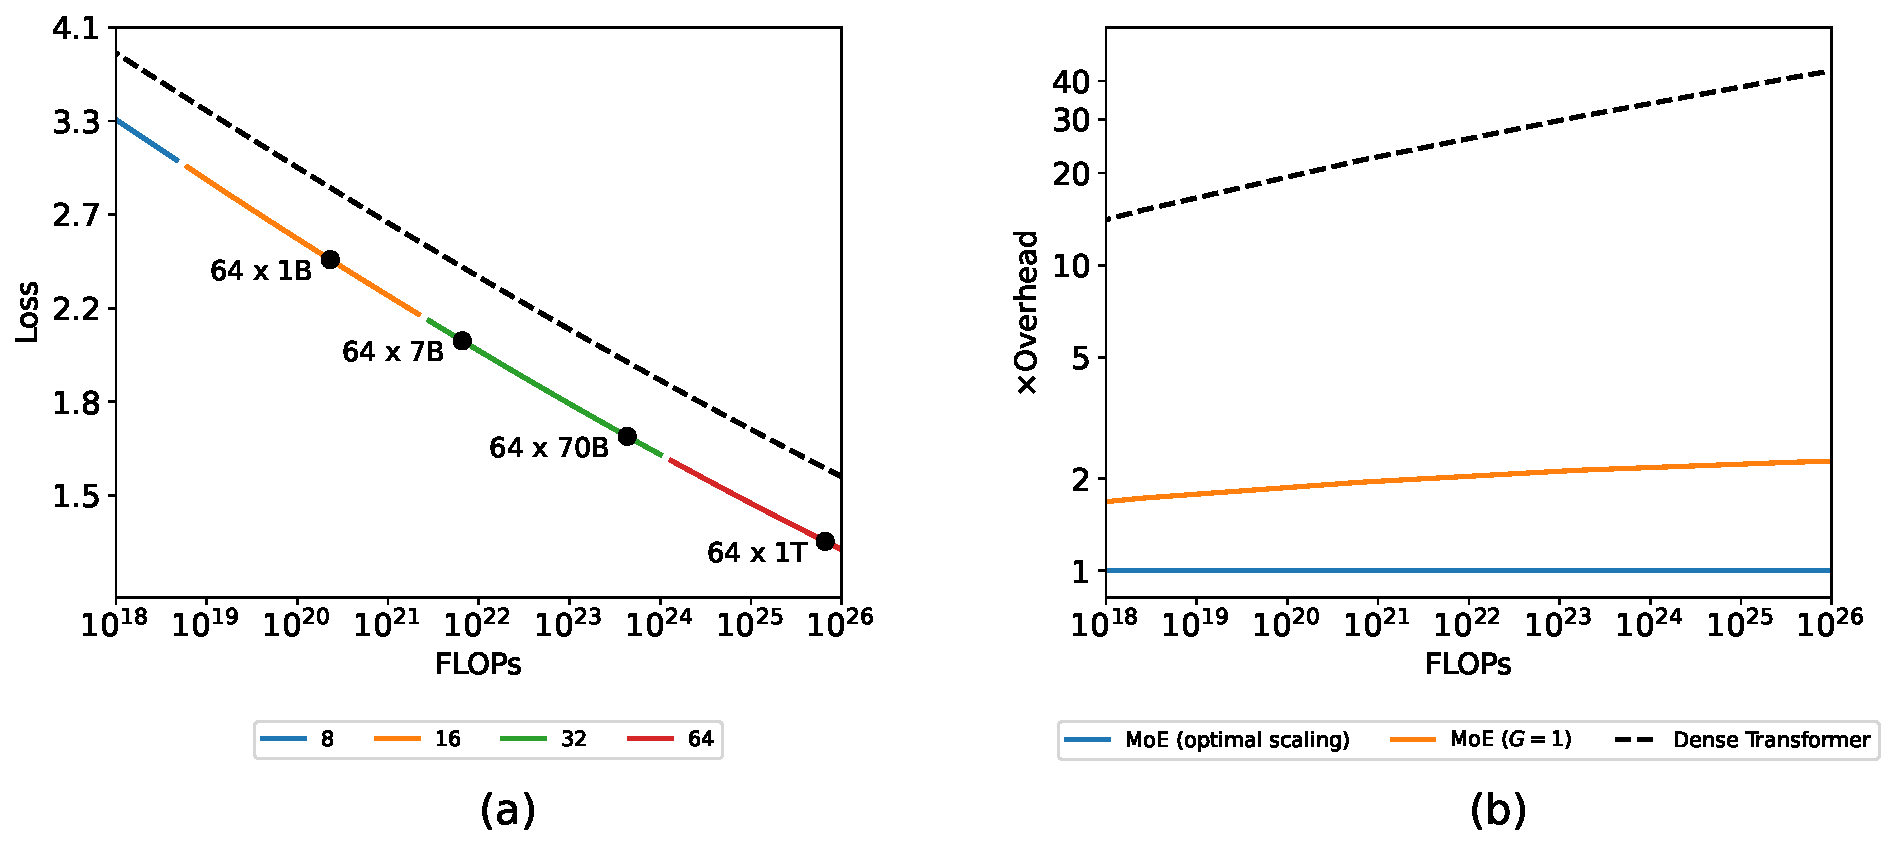
\includegraphics[width=0.99\textwidth]{figures/flags_2.pdf}
  % \medskip
  \caption{Mixture-of-Experts can be \textit{always} considered more efficient than dense Transformers, regardless of the model size. \textbf{(a)} Compute Optimal scaling curves for MoE and standard Transformers. The dashed line represents a dense Transformer. Colors denote optimal granularity for the given FLOPs training budget. \textbf{(b)} Relative number of FLOPs needed to train Transformer and Vanilla MoE (MoE with $G=1$) to achieve the performance of MoE with compute optimal $G$.}
  \label{flag_plots}
\end{figure*}
\textbf{Mixture of Experts. \ \ } 
In the context of language modeling, MoE was first introduced by \cite{shazeer2017outrageously} as a sparsely gated layer between stacked blocks of LSTM \citep{hochreiter1997long}. A similar technique was proposed in the context of Transformers by \cite{shazeer2018meshtensorflow} and \cite{lepikhin2020gshard}. \cite{fedus2022switch} proposed to route each input to only a single expert and designed a modified initialization scheme to reduce training instability.
% A similar technique was proposed in the context of Transformers by \cite{shazeer2018meshtensorflow} and \cite{lepikhin2020gshard}. These works also considered improvements in implementation and infrastructure allowing for efficient training of the gated networks. \cite{fedus2022switch} proposed to route each input to only a single expert and designed a modified initialization scheme to reduce training instability. This allowed to train models with over 1 trillion parameters and achieve 7x speedup in the pretraining speed over the dense baseline. \jk{dorzucić Artexte i tą pracę co cytuje Sebastiana}
Numerous studies have proposed to modify the original routing method. \cite{lewis2021base} used a linear assignment algorithm to postprocess token-expert mappings and ensure even expert selections. \cite{roller2021hash} suggested another approach involving deterministic hash functions. \cite{zhou2022mixtureofexperts} proposed expert choice routing, eliminating the need for additional load balancing losses. \cite{puigcerver2023sparse} designed a fully-differentiable Soft MoE architecture.


% Numerous works proposed to modify the original routing algorithm addressing its weaknesses, including load imbalance and expert under specialization. \cite{lewis2021base} used a linear assignment algorithm to postprocess token-expert mappings and ensure even expert selections. \cite{roller2021hash} suggested another approach involving deterministic hash functions. \cite{zhou2022mixtureofexperts} proposed expert choice routing instead of token choice, used originally in \cite{shazeer2017outrageously} and \cite{fedus2022switch}. This solution eliminated the need for additional load balancing losses and guaranteed balanced assignments. All of the operations used in this approach are efficiently parallelizable on modern GPU accelerators. \cite{puigcerver2023sparse} designed a fully-differentiable soft routing.
% \jk{To też można odchudzić}More recently, several open source MoE models have been released, expanding research opportunities and stimulating exploration in the community. \cite{openmoe2023} trained a 1.1T parameters model, also providing access to the intermediate checkpoints for the purpose of research. \cite{jiang2024mixtral} released Mixtral, surpassing or matching LLaMA 2 70B \cite{touvron2023llama2} and GPT-3.5 across many benchmarks. 
Concurrently to our work, \cite{dai2024deepseekmoe} proposed to modify the MoE layer by segmenting experts into smaller ones and adding shared experts to the architecture. Independently, \cite{liu2023unified} suggested a unified view of sparse \ff{} layers, considering, in particular, varying the size of memory blocks. Both approaches can be interpreted as modifying granularity.  However, we offer a comprehensive comparison of the relationship between training hyperparameters and derive principled selection criteria, which they lack.

%\sj{rephrase to state how we do better than them, not how they do worse than us. phrase us as an improvement}However, they do not present a comprehensive comparison of the relationship between training hyperparameters and lack principled selection criteria for a specific setting. \jk{druga wersja:}
%Instead, they select granularity in a rather arbitrary way.
% In the context of deep learning, MoE is built via layers that include multiple sub-networks (experts) specializing in different inputs. MoE layers gained significant popularity as an efficient way to increase the capacity of deep neural networks without increasing its inference costs, initially applied to LSTM models~\citep{shazeer2016outrageously}, and later in transformers~\citep{lepikhin2020gshard}. MoE, however, suffered from training instabilities which have been improved by selecting only one expert ~\cite{zhou2022mixture} and balancing expert load ~\cite{fedus2022switch}.  MoE models have also favorable properties in the context of the scaling laws.
% Large Language Models are widely known to benefit from high parameter count \cite{kaplan2020scaling,hoffmann2022training}, however, using all the parameters for calculating the output for each token may \mk{Czemu may, a nie po prostu result} result in unnecessarily high computational costs . In large Transformers, the \ff{} layer constitutes the majority of parameters and FLOPS and has thus become the focus of MoE-like architectural modifications. MoE in Transformer typically involves replacing the \ff{} layer with $e$ copies of itself (experts), along with a router, which handles the assignment of tokens to experts. Various 
% Most Transformer-MoEs belong to one of two categories, \textit{Token Choice} (each token is routed to a constant number of experts, e.g. \cite{shazeer2017outrageously}) or \textit{Expert Choice} (each expert receives a constant number of tokens). 
% Expert Choice (EC) is a newer technique, which achieves a better balance and faster convergence. The advantages, however, come at a price - it is not compatible with autoregressive decoding or with the batch size being different in training and inference.
% In our work, we measure the impact of granularity on autoregressive Expert Choice decoder-only models, which naturally raises the question of the applicability of the findings techniques to Token Choice architectures. We show that our findings apply to Token Choice as well, by showing that Expert Choice layers can be quickly fine-tuned to be utilized as Token Choice layers.
% MoE architectures route different inputs or parts of the input to distinct submodules. 
% 1. trochę historii i co many na myśli, 2. MoE w różnych architekturach (RNN, Transformer, etc.), 3. MoE w Transformerach - TC i EC, 4. MoE w open modelach
% \subsection{Scaling Laws}
% \paragraph{Scaling laws.} 

% \newpage
\textbf{Scaling laws.} \ Scaling laws are empirically derived equations relating the loss of a model with variables such as the number of parameters, training samples, or the computational budget. In the case of dense Transformers, scaling laws were first studied by \cite{kaplan2020scaling}, who observed power law relationships between the final model perplexity and model and dataset size. This work was extended by \cite{hoffmann2022training} by considering variable cosine cycle lengths and formulating a modified functional form of the scaling equation.
% \begin{figure*}[t]
%   \centering
%   \begin{tabular}{ c @{\hspace{30pt}} c }
%     \includegraphics[width=.43\textwidth]{icml2024/figures/plot_scaling.pdf} &
%       \includegraphics[width=.43\textwidth]{icml2024/figures/flops_save_2.pdf} \\
%     \small \textbf{(a)} &
%       \small \textbf{(b)}
%   \end{tabular}
%   \medskip
%   \caption{Mixture-of-Experts can be \textit{always} considered more efficient than dense Transformers, regardless of the model size. \textbf{(a)} Compute Optimal scaling curves for Granular models and standard Transformers. The dashed line represents a dense Transformer. Colors denote optimal granularity for the given FLOPs training budget. \textbf{(b)} Relative number of FLOPs needed to train Transformer and Vanilla MoE (MoE with $G=1$) to achieve the performance of MoE with compute optimal $G$.}
%   \label{flag_plots}
% \end{figure*}

Scaling laws have also been proposed for other architectures and training scenarios. \cite{henighan2020scaling} studied autoregressive modeling across various modalities, while \cite{ghorbani2021scaling} considered machine translation. \cite{frantar2023scaling} explored the impact of pruning on vision and language Transformers, deriving optimal sparsity for a given compute budget. \cite{clark2022unified} studied the scaling of MoE when changing model size and number of experts on a fixed dataset, concluding that routed models are more efficient only until a certain model size. In this work, we challenge that claim by considering a variable, optimal dataset size for both model families (see Section~\ref{moe_more_eff}).

% with improved scaling predictions presented in \cite{hoffmann2022training}. The extension of scaling laws to MoE-based LLMs was presented in \cite{clark2022unified}. In our work we incorporate into scaling laws granularity and the number of training tokens which allows us to achieve a better fit of the scaling laws. \jk{tu na pewno sparse scaling laws; tez inne scaling laws bylyby fajne}
%Scaling laws are of utmost practical importance, as through their extrapolation, one can justify the choice of the optimal hyperparameters of a model.
% Scaling laws have been studied in relation to MoE LLMs \cite{clark2022unified}.
% Our work differs from the previous analysis 
% %\cite{clark2022unified} 
% in the following ways:
% \begin{enumerate}
%     \item We introduce the notion of granularity and study its impact
%     \item We consider the number of training tokens 
%     \item We are more correct \sj{this needs to have better phrasing} \maciej{}
% \end{enumerate}

\section{Background}
\label{background}



\subsection{Model Architecture}
% \paragraph{Transformer.} A typical decoder-only Transformer \cite{radford2018improving, noauthororeditor, kaplan2020scaling, brown2020language} consists of an embedding layer, a stack of alternating attention and \ff{} layers, and an unembedding layer. Let $T$ be the transformer model. In the model $T$ each input token is converted by the embedding layer into a vector of size $\dmodel$, the dimension maintained across all the layers of the Transformer.

\paragraph{Transformer.} A standard decoder-only Transformer \citep{radford2018improving, noauthororeditor, kaplan2020scaling, brown2020language} consists of an embedding layer, a stack of alternating attention and \ff{} layers, and an unembedding layer. In the model, each input token is converted by the embedding layer into a vector of size $\dmodel$, the dimension maintained across all the layers in the residual stream.

The \ff{} component consists of two linear transformations and a nonlinearity $\phi$ in between. It can be described as
    $\text{FFN}(x) = \phi(xW_1+b_1)W_2+b_2$,
with $W_1$ mapping from $\dmodel$ to $\dff$, and $W_2$ back to the original $\dmodel$. It is standard \citep{radford2018improving, rae2022scaling, touvron2023llama, jiang2023mistral} to set the hidden dimension as $\dff = 4 \cdot \dmodel$. %Denote this standard dimension as $\dffbase$.

Feed-forward layers contain the majority of Transformer parameters and require the biggest computational budget counted in terms of FLOPs. Subsequently, they are the main focus of the Mixture of Experts models considered in this work.
% The \ff{} component is composed of two matrices ($W_1 \in \mathbf{R}^{\dmodel \times \dff}, W_2 \in \mathbf{R}^{\dff \times \dmodel}$) and a non-linear function such as ReLU, where $\dff$ is the size of the inner layer of a Transformer \ff{} layer. Consider $\dffbase$ to be the size of the inner layer of the feed-forward layer in the standard setting, that is $\dff=\dffbase$. Then, typically $\dffbase=4\dmodel$ \ka{cite}.  This setting results in the number of parameters in the layer, $\pff = 8\dmodel^2$. 

% The \ff{} component is composed of two matrices ($W_1 \in \mathbf{R}^{\dmodel \times \dff}, W_2 \in \mathbf{R}^{\dff \times \dmodel}$) and a non-linear function such as ReLU, where $\dff$ is the size of the inner layer of a Transformer \ff{} layer. Consider $\dffbase$ to be the size of the inner layer of the feed-forward layer in the standard setting, that is $\dff=\dffbase$. Then, typically $\dffbase=4\dmodel$ \ka{cite}.  
% This setting results in the number of parameters in the layer, $\pff = 8\dmodel^2$. 
\paragraph{Mixture of Experts.} 
% The main idea behind MoE in Transformer is to replace each \ff{} layer with $\nexpert$ \ff{} layers (\textit{experts}) and route each token to only a subset of the experts. In MoE, the inner dimension of each expert network is $\dff$, the size of the base model $T$. In this design, the parameter count of a MoE layer scales linearly with the number of experts, $\pmoe = \nexpert \cdot \pff.$.
The core idea behind MoE in Transformers is to replace the feed-forward layer with a set of $\nexpert$ \textit{experts}. The size of each expert is typically \citep{fedus2022switch, zhou2022mixtureofexperts, zhou2023brainformers, jiang2024mixtral} set to mirror the original dimensions of the layer, with the hidden expert dimension $\dexp{}$ equal to $\dff.$ Therefore, the total number of parameters in MoE scales linearly with the number of experts. 
%However, the number of \textit{active} parameters (i. e. parameters used to produce output for a single token) remains constant.
However, the computational cost remains approximately constant as each input is routed and then processed by a subset of experts.
% resolved: \kk{Wspomniec ze uzywamy expert-choice i ze mamy softmax po batchu i sugestia od Sebastiana zeby w appendixie zrobic shading na oryginalnych autorow ze jedynie wspominaja o softmaxie po batchu w odpowiedzi na review}
% Originally Mixture of Experts (MoE) posits that each token \textit{selects} the most appropriate expert for its processing \ka{cite}. However, this method, termed \textit{token-choice}, exhibits certain limitations, such as load imbalance and a fixed computational cost for each token. To overcome these drawbacks, our research adopts the \textit{expert-choice} routing strategy \cite{zhou2022mixtureofexperts}, with minor adjustments to ensure compatibility with autoregressive decoding.  In our architecture, each expert chooses $k$ tokens from all tokens in the input batch, sharing the position in the input sequence (tokens are chosen across the batch dimension).

\newpage
\subsection{Scaling Laws}
\label{sec:back_scaling}

\textbf{Dense Transformers.} Large Transformer-based models are known to approximately obey the power-law relationship between final loss $\mathcal{L}$, model size $N,$ and number of training tokens $D.$ This relationship is often called {\it Chinchilla scaling laws} described by \cite{hoffmann2022training} as
\begin{align}\label{eq:chinchilla}
    \mathcal{L}(N, D) = c + \frac{a}{N^\alpha} + \frac{b}{D^\beta}. 
    % L(N,D) - e - \frac{b}{D^\beta} = \frac{a}{N^\alpha} \\
    % log(L(N,D) - e - \frac{b}{D^\beta}) = log(\frac{a}{N^\alpha})
\end{align}


The power-law formula is composed of three distinct terms that characterize the intrinsic entropy of data, constraints of the model, and limitations in the training data. The term $c$ represents the minimum possible error intrinsic to the data. The remaining two terms are suboptimality terms, which address the limitations in function representation owing to the size of the model and in data signified by the number of tokens. In the limit, with infinite data and model size, the loss is reduced to $c$.

%The first term in this equation represents the entropy inherent to the modeled distribution, while the second and third term capture the difference between a perfect model with with a finite one trained on a given number of tokens. \\


\textbf{Mixture of Experts.}  For MoE Transformer-based models, \cite{clark2022unified} formulated the final loss for a constant dataset size \( D \) of 130B tokens, allowing for variations in the expansion rate \( E \), as: 
\begin{align}\label{eq:scaling_law}
    \mathcal{L}(N, E) = \left( \frac{10^{d/a}}{N}\right)^a \left( \frac{1}{E}\right)^{b+c\log{N}}.
\end{align}

However, this result has a notable limitation as it can be applied only to the original dataset size. The scalability and effectiveness are constrained in this scenario because it is crucial to align the number of training samples with the available computational resources for optimal use. As per \cite{kaplan2020scaling} and \cite{hoffmann2022training}, maintaining a constant dataset size while scaling up the neural network size leads to undertraining, resulting in a model that does not perform to its full potential.


% leads to a number of problems, such as load imbalance

% having a set $\nexpert$ \ff{} layers (\textit{experts}) and t
% In the standard setting \kk{cite?}, each MoE \ff{} layer in a Transformer consists of  $\nexpert$ \ff{} layers (\textit{experts}), each the same size as a regular \ff{} layer ($\dff=4\dmodel$) along with a \textit{router}, a component performing the assignment of tokens to experts.

% is constructed by creating a set of \textit{experts}, each having the size of a regular \ff{} layer. The number of parameters $\pmoe$ in the layer scales proportionally with the number of experts $e$,
% \begin{align*}
    % \pmoe = e \cdot \pff,
% \end{align*}
% where $\pff$ is the number of parameters in the base feed-forward layer \mk{wydaje mi się że nie wiadomo czym jest base feed-forward layer?}.
% The computational load is maintained at a roughly consistent level through the activation of a selected subset of parameters for each distinct input. This architecture allows for scaling predominantly by incorporating additional experts of equivalent dimensions. The amount of computation can be adjusted by changing the \textit{capacity factor} that controls the amount of input data received by each expert. 

% The expected number of tokens routed to each expert, denoted by $k$, is calculated according to the equation 
% \begin{align*}
    % k = \frac{c}{e} \cdot b,
% \end{align*}
% where $c$ is the capacity factor, $b$ is the total number of tokens in the input batch, and $e$ is the number of experts.

% In our research, we suggest an alternative approach where the hidden dimension of the expert is not set to mirror that of the base feed-forward layer, but is instead fine-tuned to a value that might be more effective. This approach allows the configuration of the Mixture of Experts (MoE) to be articulated in terms of two key parameters: \textit{granularity} (\(G\)) and \textit{expansion rate} (\(E\)).

% Let's \mk{let us denote?} denote $\dff$ as the hidden dimension of the base feed-forward layer and $\dexpert$ as the hidden dimension of a single expert. Granularity is defined as 
% \begin{align*}
    % G = \frac{\dff}{\dexpert}, 
% \end{align*}
% while expansion rate is the proportion 
% \begin{align*}
    % E = \frac{\pmoe}{\pff}.
% \end{align*}


% show that in order to optimally train models with ever increasing computational budget, both the amount of data and the size of the model should be scaled up. However, usually, the number of the Floating Point Operations (FLOPs) needed to run inference



% \textbf{Mixture of Experts}  Mixture of Experts \mk{powtórzenie?} (MoE) describes a number of related machine learning architectures that rely on conditional computation. In the original formulation \cite{moe1991} it denoted an ensemble-like architecture in which a single \textit{expert} model out of many is run for a specific input, with a separate, computationally inexpensive \textit{router model} selecting the most suitable expert.

\section{Granularity}


As described in Section~\ref{background}, in the standard setting, the inner dimension of each expert network, $\dexp$, is equal to $\dff$, which is the same size as the \ff{} layer of the base model.
\begin{figure*}[t]
  \centering
  \begin{tabular}{ c @{\hspace{30pt}} c }
    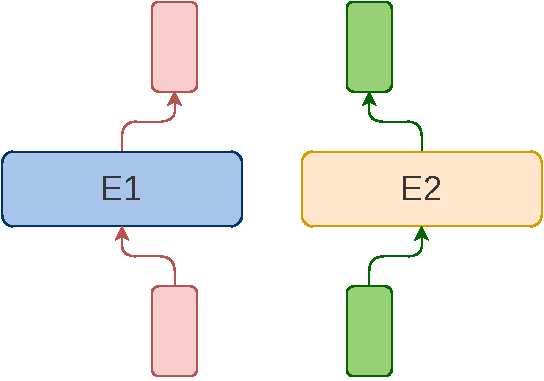
\includegraphics[width=.45\textwidth]{figures/diagram_left_2.pdf} &
      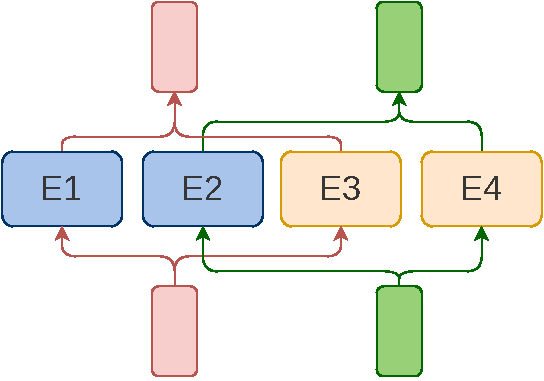
\includegraphics[width=.45\textwidth]{figures/diagram_right_2.pdf} \\
    \small \textbf{(a)} &
      \small \textbf{(b)}
  \end{tabular}

  \medskip

  \caption{\textbf{(a)} Standard MoE layer with $G=1$ \textbf{(b)} Corresponding MoE layer with $G=2$. Each of the original experts is split into two granular ones. The split occurs in the hidden dimension of an expert. Increasing $G$ allows for a more precise mapping between experts and tokens. Since for granularity $G$, the token is routed to $G$ granular experts, the number of parameters activated per token is the same in both cases.}
  \label{diag_gran_better}
\end{figure*}





In this work, we suggest an alternative approach where the hidden dimension of the expert is not necessarily set to mirror that of the standard feed-forward layer. Instead, it can be adjusted to a value that is the most effective. This approach allows the configuration of MoE to be articulated in terms of two key hyperparameters: \textit{granularity} (\(G\)) and \textit{expansion rate} (\(E\)). In the following parts of this work, we will also use the term \textit{active} parameters to refer to the non-embedding parameters used to produce output for a single token, except routing. The number of active parameters is denoted as $\nact$.

Let $\dexpert$ be the hidden dimension of a single expert. Granularity is defined as
\begin{align*}
    G = \frac{\dff}{\dexpert}.
\end{align*}
In other words, granularity denotes the multiplier factor for the change in the size of an expert from the original standard model, defined as $G=1$. 
In this work, we investigate $G > 1$ where experts are smaller than in the standard layer. 

Note that increasing granularity does not affect the number of active parameters. As $G$ increases, the number of experts that process the token grows proportionally to $G$. In other words, for granularity $G$, a token is routed to $G$ fine-grained experts, thereby keeping the number of active parameters constant. See Fig. \ref{diag_gran_better} for visualization.

We then define the \textit{expansion rate}, which describes the increase in the number of parameters from a standard transformer layer to a MoE layer. Given that, $\nmoe$ and $\nff$ denote the total number of parameters in a MoE layer excluding routing and the standard \ff{} layer, respectively. The expansion rate $E$ is then defined as 
\begin{align*}
    E = \frac{\nmoe}{\nff}.
\end{align*}

Expansion rate can also be seen as the total number of parameters in a MoE layer compared to its active parameters. 

The concept of the expansion rate is intricately linked to the number of experts through the idea of granularity. Indeed, the definitions of both granularity and expansion rate extend and refine our understanding of the number of experts, symbolized as $\nexpert$.
\begin{align}
    \nexpert = G \cdot E
\end{align}

For non-granular models, where $G=1$, the expansion rate is equal to the number of experts. 



Intuitively, increasing granularity for a given expansion rate gives the model more flexibility in mapping datapoints to experts, potentially improving performance. We incorporate the notion of granularity into our scaling laws in Section~\ref{sec:scaling_laws}. The discussion about practical tradeoffs in changing this parameter is given in Section~\ref{sec:scaling_app}.



\section{Scaling Laws}\label{sec:scaling_laws}

% It has been known that transformer model performance has a power-law relationship with the factors: model size (N), dataset size (D) \cite{kaplan2020scaling, hoffmann2022training}. In this section, we factorize granularity as the new dimension and show how it also follows the scaling law.

Granularity determines changes in the architecture of MoE. In this section, we answer a central question of this work: whether the granular MoE models follow scaling laws and, if so, how granularity affects them. Thus, we aim to derive a parametric scaling law for predicting the final loss value $\mathcal{L}$ based on granularity $G$, total number of non-embedding parameters $N$, and number of training tokens $D$. 

% \begin{figure}[t]
% \centering
% \includegraphics[width=0.5\textwidth]{icml2024/figures/delta.pdf}
% \caption{
% Difference in the loss between training for 16B and 65B tokens for all model sizes and granularity values.
% % \marekc{I suggest to compress the model sizes to a human readable format} \janek{TODO: tak}
% }
% \label{fig:gran_project_no_interact}
% \end{figure}

% \begin{figure}[t]
% \centering
% \includegraphics[width=0.4\textwidth]{icml2024/figures/granularity_N_1082130432_D_31250.0.pdf}
% \caption{
% We plot the effect of $G$ on $\mathcal{L}_{N,D}(G)$ for constant $N$ and $D$. Both axes are in the log-scale. The results suggest the linear relationship between $\log(G)$ and $\log(\mathcal{L}-c)$.
% The given values are $N=64 \times 25M$, $D=16B$, $const=3.12$ .  The plots for additional values of $N$ and $D$ can be found in Appendix \ref{sec:app_add_viz}.
% % \marekc{I suggest to compress the model sizes to a human readable format} \janek{TODO: tak}
% }
% \label{fig:loss_nd_g}
% \end{figure}

% \begin{figure*}[t]
%   \centering
%   \begin{tabular}{ c @{\hspace{2pt}} c @{\hspace{10pt}} c}
%     \includegraphics[width=.3\textwidth]{icml2024/figures/granularity_N_1082130432_D_31250.0_new_ratio.pdf} &
%         \includegraphics[width=.302\textwidth]{icml2024/figures/kaplan_4.pdf} &
%             \includegraphics[width=.33\textwidth]{icml2024/figures/delta.pdf} \\
%     \small \textbf{(a)} &
%       \small \textbf{(b)} &
%         \small \textbf{(c)} &
%   \end{tabular}

%   \medskip

%   \caption{\textbf{(a)} We plot the effect of $G$ on $\mathcal{L}_{N,D}(G)$ for constant $N$ and $D$. Both axes are in the log-scale. The results suggest the linear relationship between $\log(G)$ and $\log(\mathcal{L}-c)$.
% The given values are $N=64 \times 25M$, $D=16B$, $const=3.12$ .  The plots for additional values of $N$ and $D$ can be found in Appendix \ref{sec:app_add_viz}. \textbf{(b)} The impact of varying the number of parameters $N$ on the loss for fixed granularity $G=4$. For other granularity values, see Appendix \ref{sec:app_add_viz}. \textbf{(c)} The difference in the loss between training for 16B and 65B tokens for all model sizes and granularity values. The model size is reported as the expansion rate and the number of active parameters.}
%   \label{empirical}
% \end{figure*}

We run over 100 experiments on the decoder-only Transformer architecture, with each \ff{} component replaced by a Mixture of Experts layer. Those experiments involve training models with sizes ranging from 129M to 3.7B parameters across different training durations, from 16B to 130B tokens. We consider logarithmically spaced values of granularity between 1 and 16. To constrain the search space, $E=64$ is fixed, following the recommendations of \cite{clark2022unified}.  In addition, we also run experiments with dense Transformers to compare their performance with MoE. The details of all architectures, the training procedure, and hyperparameter choices are described in detail in Appendix~\ref{app:setup}.

% \newpage
In the subsequent part of this paper, we will use the notation $E\times \nact$ to describe a MoE model with $\nact$ active parameters and expansion rate $E.$

% \begin{figure}[t]
% \centering
% \includegraphics[width=0.45\textwidth]{icml2024/figures/kaplan.pdf}
% \caption{
% Experimental results for a fixed granularity. Both axes are in log scale \ka{experiments for other granularities in appendix?}.
% % Scaling model and dataset size for a fixed granularity. We observe close to linear relationship in the log-log scale, which implies power law in both parameters. Dashed lines are fitted to each set of points separately for the purpose of illustration.
% } 
% \label{scaling_n_d}
% \end{figure} 
% \begin{table}[h]
%     \centering
%     \begin{tabular}{c|c}
%         \# Parameters & 25M, 50M, 100M \\
%         \hline
%         \# Training tokens & 25M, 50M, 100M \\ 
%         \hline
%         \# Granularity & 25M, 50M, 100M \\ 
%         \hline
%         \# Total runs & 25M, 50M, 100M \\ 
%     \end{tabular}
%     \caption{Compute optimal training hyper-parameters for MoE models. \sj{This importantly should have flops on the left.}}
%     \label{tab:compute_opt}
% \end{table}

% In this section we derive and validate scaling laws for MoE considering granularity, model size and number of training tokens. The details of the training setup, routing algorithm used, etc. are presented in \ref{sub:setup}.

%The star

% \begin{figure*}[ht!]
% \centering
% \includegraphics[width=0.8\textwidth]{icml2024/figures/gran_sep.png}
% \caption{Granular MoE models empirically obey similar power-law scaling when increasing model size, at least when hyper-parameters do not diverge too much from the optimum. Lines drawn here are just to visualize the trend, and are not generated by our scaling law, unlike other plots. \janek{check: To prawda? wydawało mi się, że ten plot tak był zrobiony} 
% \ka{labels should be bigger / more easily legible,
% also details like $10^0$ can be written only once at the top or so. saying number of tokens instead of number of steps?
% }
% }
% \label{fig:gran_linear}
% \end{figure*}


\newpage
\subsection{Power Law With Respect to Granularity} 
%To create a joint scaling laws formula for $N$, $D$ and $G$, we first need to investigate how $G$ determines loss independently for each $(N,D)$, analysing $L_{N,D}(G)$. 
We first answer the question of whether granular models follow the scaling laws. In Figure~\ref{fig:scalinglaws}(a), it can be seen that increasing granularity results in a lower loss. The returns follow approximately an exponential pattern, converging to a positive constant.   The empirical relationship given by Figure \ref{empirical}(a) suggests the following power-law dependence of loss on a varying granularity for given $N$ and $D$ and constants $g, h$ and $\gamma$ that may be dependent on them,
% As we already noted multiplicative relationship between $N$ and $G,$ we can assume the interaction
% \begin{align}
%     L_{D}(N, G) = \left(\frac{C}{G^\gamma} + c\right)\frac{1}{N^\alpha} + A.
% \end{align}
% \janek{TODO rewrite paragraphs above, using arguments from previous version and a plot. Prove that on loss/granularity plot with constant N and D we can see the following equation. I think that now it's enough to prove that this equation is correct independently for any N and D}:
\begin{align}\label{eq:g_only}
    \mathcal{L}_{N,D}(G) = \frac{g_{N,D}}{G^{\gamma_{N,D}}} + h_{N,D}.
\end{align}
%\ps{Ja nie rozumiem tej dyskusji, czy ktoś to może przepisać/rozwinać? Też $x$ jest nie wprowadzonym wcześniej oznaczeniem, więc nie jest jasne jaką rolę odgrywa.}
\begin{figure*}[t]
  \centering
  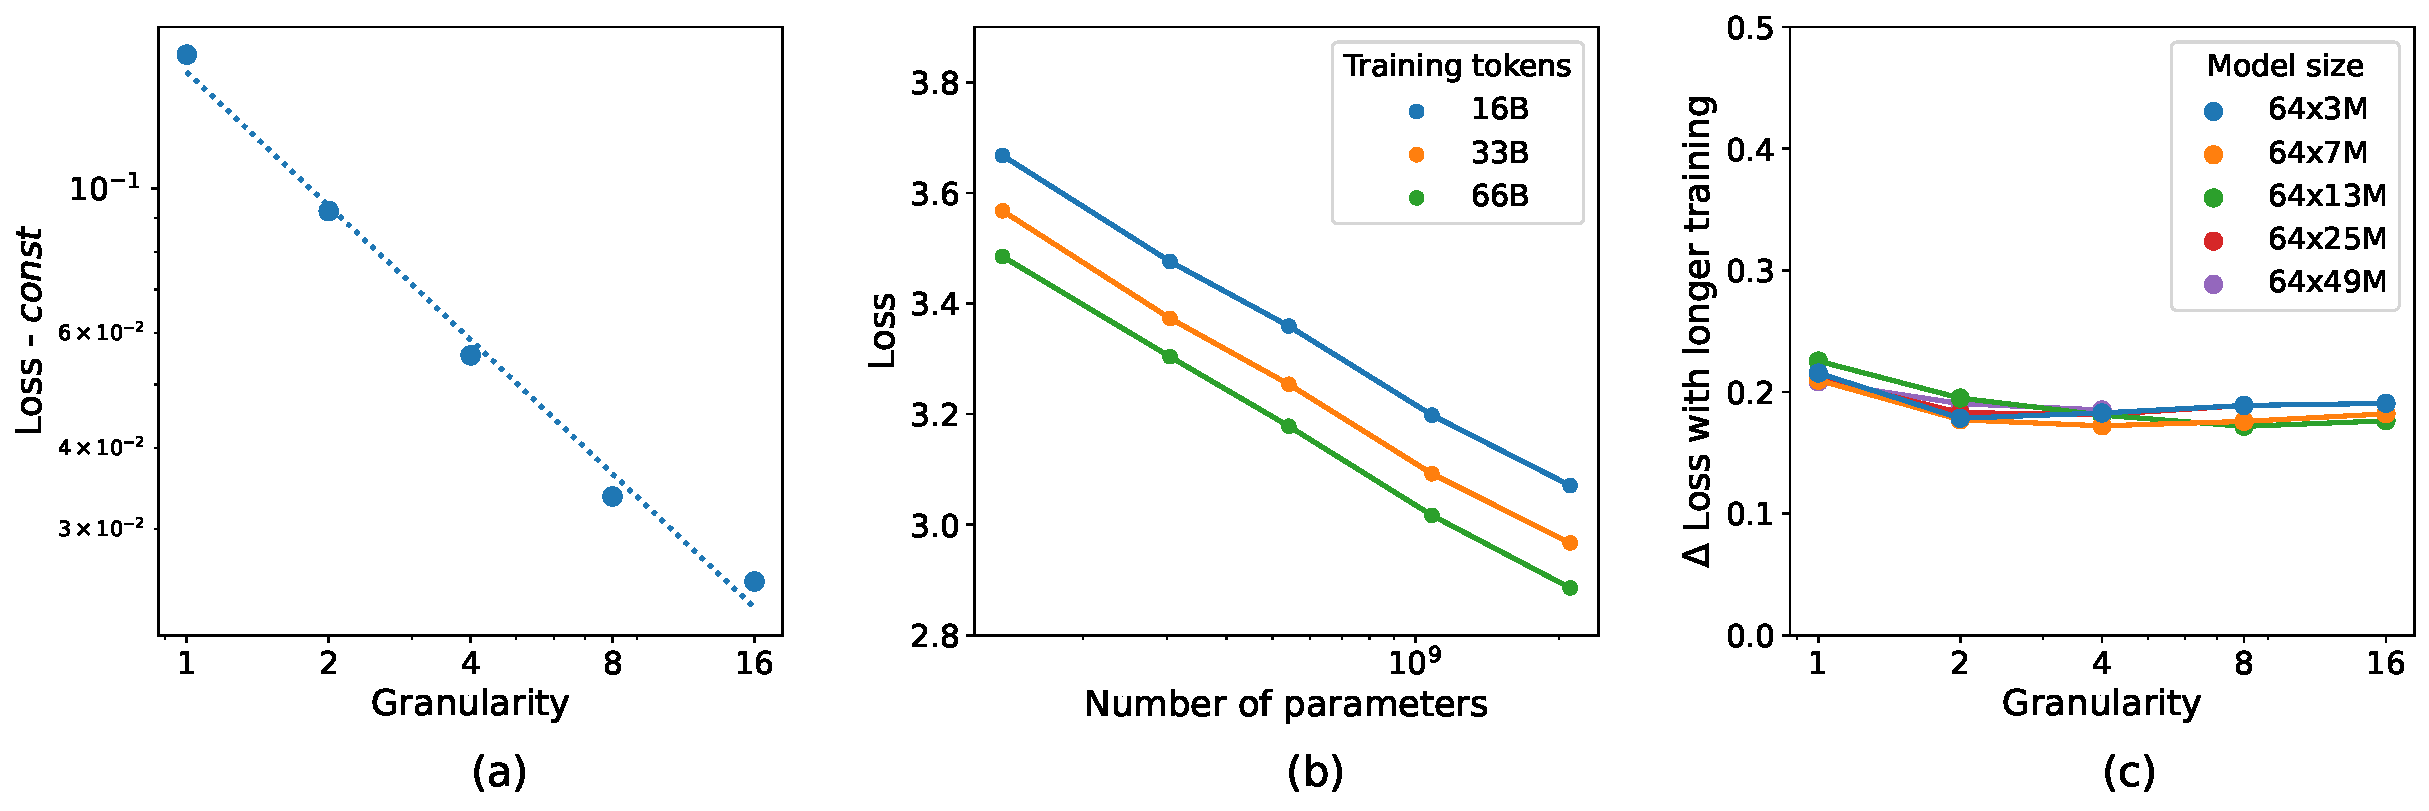
\includegraphics[width=.99\textwidth]{figures/derivation_formula.pdf}
  % \medskip
  \caption{\textbf{(a)} The effect of $G$ on $\mathcal{L}_{N,D}(G)$ for constant $N$ and $D$. Both axes are in the log-scale. The results suggest the linear relationship between $\log(G)$ and $\log(\mathcal{L}-c)$.
The given values are $N=64 \times 25M$, $D=16B$, $const=3.12$ .  The plots for additional values of $N$ and $D$ can be found in Appendix \ref{sec:app_add_viz}. \textbf{(b)} The impact of varying the number of parameters $N$ on the loss for fixed granularity $G=4$. For other granularity values, see Appendix \ref{sec:app_add_viz}. \textbf{(c)} The difference in the loss between training for 16B and 65B tokens for all model sizes and granularity values. The model size is reported as the expansion rate and the number of active parameters.}
  \label{empirical}
\end{figure*}
\subsection{Scaling the Model and Dataset Size}
\label{sec:scaling_model_data}
As outlined in Section~\ref{sec:back_scaling}, the power-law given by Eq.~\ref{eq:chinchilla} consists of three terms that describe inherent data entropy and limitations in function representation and data. This derivation is independent of the architecture. In particular, the Eq.~\ref{eq:chinchilla} also holds for constant granularity. Empirically, we observe a power law relationship in $N$ and $D$ analogous to that in dense models as depicted in Figure~\ref{empirical}(b) for a fixed value of granularity (see also Fig.~1, \cite{kaplan2020scaling}).  Furthermore, the validity of this functional form is verified by fit in Section~\ref{sub:parametric}. 

Since we know that separate scaling laws are valid for given granularities, in the general form, the parameters in Eq.~\ref{eq:chinchilla} can be dependent on the model's granularity:
\begin{align}\label{eq:gran_func}
     \mathcal{L}_G(N, D) = c_G + \frac{a_G}{N^{\alpha_G}} + \frac{b_G}{D^{\beta_G}}.
\end{align}


%In order to obtain an equation modeling the loss for a fixed granularity, we can follow the discussion presented in~\cite{hoffmann2022training}. Despite changes in the architecture in MoE models, the size of the hypothesis space depends on the number of parameters. Similarly, the stochastic approximation term is determined by the dataset size. Therefore, we expect Eq.~\ref{eq:chinchilla} to also hold in this context. 

% \jk{poprzedni tekst poniżej:}
% In our experiments, we empirically observe that the power-law given by Eq.~\ref{eq:chinchilla} also holds for granular models. Empirical observations reveal a linear relationship between the logarithm of the loss function and the logarithm of the number of non-embedding parameters, consistent across varied granularity and token counts. Fig. \ref{scaling_n_d}, on a log-scale depicts a linear relationship between the number of parameters $N$ and the loss $L$ for constant granularity. The linear relationship holds for multiple values of the number of tokens $D$ whose impact is incorporated into the constant of the linear equation. Fig~\ref{scaling_n_d} presents the analogous case where the linear relationship holds between the loss and the number of tokens.

\subsection{The Form of the Joint Scaling Law}\label{sub:joint}


%The key question of this work is how granularity $G$ can follow scaling laws.  %Below we make several observations on the restrictions on the formula and derive its final form. 
Following the above observation that models with constant granularity obey Chinchilla scaling laws given by Eq.~\ref{eq:chinchilla}, the key question arises as to how the general notion of granularity $G$ can be incorporated into the joint scaling law. %, sharing the formula across all granularities.
Moreover, the scaling law formula from Eq.~\ref{eq:gran_func} for constant $N$ and $D$ has to be representable by Eq. \ref{eq:g_only}. This is because the former is a more general equation, encompassing shared hyper-parameters across all $N$, $D$, and $G$. It is anticipated to align with the latter, consisting of distinct power laws, each with specific parameters for different $N$ and $D$ values. Consequently, the objective is to identify a function that fulfills these criteria.

%because the former is a more general equation, sharing hyper-parameters for all $N$, $D$ and $G$ and we should expect that it matches the latter, which represents set of separate power laws, with specific parameters for each $N$ and $D$ \sj{that sentence is way too long and complicated}. \jk{podoba mi się to zdanie, można je jednak podzielić} This means, that we want to find a function that satisfies: 
\begin{align}\label{eq:l_general}
% \begin{array}{lll}
     \mathcal{L}(N, D, G) &= \hspace{0.43cm} \mathcal{L}_{N,D}(G)  \hspace{0.43cm} = \hspace{0.6cm} \mathcal{L}_G(N,D) & \\
      &= \frac{g_{N,D}}{G^{\gamma_{N,D}}} + h_{N,D} = c_G + \frac{a_G}{N^{\alpha_G}} + \frac{b_G}{D^{\beta_G}} & \nonumber
% \end{array}
\end{align}
%In general form, the parameters in Eq.~\ref{eq:chinchilla} are assumed to be functions of the model's granularity:
%\begin{align}\label{eq:gran_func}
     %L_G(N, D) = C_G + \frac{A_G}{N^{\alpha_G}} + \frac{B_G}{D^{\beta_G}}.
%\end{align}
%\begin{align}\label{eq:gran_func}
 %   L(N, D, G) = L_0' + \frac{a}{N(G)^{\alpha}} + \frac{b}{D(G)^{\beta}} +G(G),
%\end{align}

% \begin{align}\label{eq:gran_func}
%     L(N, D, G) = L_0(G) + \frac{A(G)}{N^{\alpha(G)}} + \frac{B(G)}{D^{\beta(G)}}.
% \end{align}
In the subsequent sections, we aim to determine which of these parameters remain independent of $G$ and identify their functional form. Furthermore, we present some rationale for the structure of our formula.


\textbf{Lower Bound.}
Consider the limit of Eq.~\ref{eq:gran_func} for $N$ and $D$ growing to infinity:
\begin{align}\label{eq:gran_limit}
\lim_{\substack{N\to \infty\\ D\to \infty}}    \mathcal{L}(N, D, G) = c_G.
\end{align}
% As argued in Sec. \ref{sec:scaling_model_data}, the bound of the achievable loss when training bigger models on more samples should not be dependent on the architecture. Hence, 
% we get $\mathcal{L}_0(G) = L_0$, and 
% One possible solution is to include $G$ as an individual factor, with a similar role to $N$ and $D.$ This would lead to the equation
% \begin{align}\label{eq:gran_summand}
%     L(N, D, G) = L_0' + \frac{C}{G^\gamma} + \frac{A(G)}{N^{\alpha(G)}} + \frac{B(G)}{D^{\beta(G)}}.
% \end{align}
% %\marekc{Perhaps we write "with growing $N$ and $D$ the loss converges to" instead of "reduces to"?} 
% Note however that with growing $N$ and $D$ and a fixed $G$, Equation \ref{eq:gran_func} converges to
% \begin{align}\label{eq:gran_summand_const}
%     L_G(N, D) = L_0' + L_G + \frac{A'}{N^{\alpha'}} + \frac{B'}{D^{\beta'}},
% \end{align}
% \begin{align}\label{eq:gran_summand_const}
%     L_0(G) = L_0' +  \frac{C}{G^\gamma} 
% \end{align}
 with the constant term $c_G$ dependent on granularity. This is contradictory to the fact that it captures the inherent entropy of the dataset. Lower bound of the achievable loss when training bigger models on more samples should not depend on the architecture, therefore parameter $c_G=c$ is constant for all granularities. 
%the expected form of the equation can be reduced to
%\begin{align}\label{eq:}
%    L(N, D, G) = L_0 + \frac{a}{N(G)^{\alpha'}} + \frac{b}{D(G)^{\beta'}},
%\end{align}
 %\begin{align}
     %L(N, D, G) = L_0 + \frac{A(G)}{N^{\alpha(G)}} + \frac{B(G)}{D^{\beta(G)}},
 %\end{align}
%with the second and third terms capturing interactions between granularity and the size of the model and dataset respectively. In the next part of this section, we will describe these interactions based on empirical data.
% The key problem is then understanding interactions between granularity and other parameters, that is the number of tokens $D$ and the number of parameters $N$. Fig.~\ref{fig:gran_project} describes the linear relationship between the number of parameters and loss as seen also in Fig.~\ref{scaling_n_d}. However, Fig.~\ref{fig:gran_project} presents the lines for several granularity values.




\textbf{Granularity and Number of Tokens $D$.} 
As seen in Figure~\ref{empirical}(c), the benefit of training a model on a larger dataset is almost the same for each granularity value. This suggests that there is no interaction between $D$ and $G$. Therefore, we can assume that 

%\begin{align}
    %\frac{b}{D(G)^{\beta}} = %\frac{b}{D^\beta},
%\end{align}
 \begin{align}
     \frac{b_G}{D^{\beta_G}} = \frac{b}{D^\beta}.
\end{align}

%leaving us with:
% \begin{align} \label{eq:gran_no_d}
%      L(N, D, G) = c + \frac{a_G}{N^{\alpha_G}} + \frac{b}{D^\beta}.
% \end{align}

%\begin{align} \label{eq:gran_no_d}
%    L(N, D, G) = L_0 + \frac{a}{N(G)^{\alpha'}} + \frac{b}{D^\beta},
%\end{align}

%\jk{poprzednia wersja:}
%\begin{align}
%    L(D, G) = \frac{B}{D^\beta}.
%\end{align}
%Fig.~\ref{fig:gran_project_no_interact} presents three plots for different values of the number of tokens $D$. The shapes of the presented lines in each of the plots are very similar but differ in their relative position on the vertical axis. The larger steps result in lower loss values, suggesting the number of tokens can be incorporated into the constant and does not affect the loss independently from granularity. 



% \begin{figure*}[ht!]
% \centering
% \includegraphics[width=0.6\textwidth]{icml2024/figures/final_scaling.pdf}
% \caption{We present the fit of the scaling law compared to experimental results. }
% \label{fig:scalinglaws}
% \end{figure*}

% \begin{figure*}[t]
%   \centering
%   \begin{tabular}{ c @{\hspace{5pt}} c @{\hspace{100pt}}}
%     \includegraphics[width=.725\textwidth]{icml2024/figures/final_scaling.pdf} &
%       \includegraphics[width=.27\textwidth]{icml2024/figures/validation.pdf} \\
%     \small \textbf{(a)} &
%       \small \textbf{(b)}
%   \end{tabular}

%   \medskip

%   \caption{\textbf{(a)} Fit of the scaling laws compared to the experimental results. \textbf{(b)} Validation of the fit. }
%   \label{fig:scalinglaws}
% \end{figure*}



%\jk{tak naprawdę chyba najlepiej byłoby sparafrazować to zdanie ze sparse scaling laws (mamy te same wyniki): the model size power law scaling for all granularity levels differs primarily in
%a constant factor (intercept in a log-log plot); $\alpha$ stays consistent.}
%

%\janek{Brakuje tutaj jakiegoś plota uzasadniającego, że samą zmianę granularity możemy modelować power law, przy stałych tokenach i parametrach. Nie ma też argumentu, czemu nie ma granularity nie ma w wykładniku. Coś tego typu musi sie tu znaleść: Similarly to (sparse scaling) \cite{sparsescalinglaws} we let the exponents be independent of granularity, since this would either break the simple power law relationship between granularity and perplexity or introduce too much parameters and complexity for extrapolations to be reliable and parametric fitting to be numerically stable, however we think that approach this might be a promising direction for the future, but this goes beyond the scope of this work. }






% \janek{ponizej text do przepisania na argumentacje eq 10 z L(G)}

% \textbf{Granularity and model size.} 
% In Fig. \ref{fig:parallel_better}, we see that the loss values for a varied model size form almost parallel curves, characterized by granularity. Thereby, a certain change in the value of $G$ shifts the loss by the same amount for each model size. This linear relationship on the log-log scale translates into a multiplicative interaction between $N$ and $G$. 


%\begin{figure}[ht!]
%\centering
%\includegraphics[width=0.47\textwidth]{icml2024/figures/lines_shorter_2.png}
%\caption{
%Loss values for models trained on a fixed number of tokens. Dotted lines are fit separately to each set of points for the purpose of illustration.
%\sj{Steps into tokens; parameters into 20k/20M etc., round them up/down. In general those charts seem a bit random.} \janek{I jaka tu jest skala na %osi y, to jest log?} 
%}
%\label{fig:parallel_better}
%\end{figure}

% In Fig.~\ref{fig:parallel_better} as we vary granularity logarithmically, it is evident that in the log-scale decreasing the granularity's exponent by a constant value has a varied impact on the constant in the power-law equation. 
% In other words, we observe an exponential trend in the final loss, which tends to plateau at higher granularity levels. This trend offers insights into the diminishing returns of increased granularity in model training. At the same time, this effect suggests a potential interplay between the number of parameters and granularity. 



% As we already noted multiplicative relationship between $N$ and $G,$ we can assume the interaction
% \begin{align}
%     L_{D}(N, G) = \left(\frac{C}{G^\gamma} + c\right)\frac{1}{N^\alpha} + A.
% \end{align}

%\jk{To moja wersja tego rozdziału. Poprzednią zostawiam poniżej}\textbf{Power law in granularity.} In Fig.~\ref{fig:scalinglaws} We can notice that increasing granularity results in lower loss. However, the returns are diminishing. This suggests power law dependence of loss on a varying granularity. We can incorporporate this dependence into \ref{eq:gran_func} by setting 
%\begin{align}
    %a(G)=\frac{c}{G^\gamma} + d,
%\end{align}
%leading to the following functional form of the scaling law
%\begin{align}
    %%L(N, D, G) = L_0 + \left(\frac{c}{G^\gamma} + d\right)\frac{1}{N^\alpha} + \frac{b}{D^\beta}.
%\end{align}
%\janek{potrzebujemy plota do argumentacji tej formy, który pokazuje dokładnie, jak dla paru konkretnych przykładów N i D, $L_{N,D}(G)$ wykładniczo maleje, układając się w prostą w log skali} \ps{Z czego wynika kolejne zdanie? Tutaj chyba brakuje odniesienia do Wykresu 5 i powiedznia, ze to pasuje. Co więcej jak fitujemy power-law to dobrze jak wykresy były w powójnie logarytmicznej skali tak aby były widoczne proste linie.} 

\textbf{Granularity and Model Size $N$.}  
We consider \( \alpha \) to be a constant that describes how the function scales with \( N \). In this work, we assume polynomial functional forms that rule out the potential dependency of $\alpha$ on $G$ given the form of Eq. \ref{eq:g_only}. 
%Changing \( \alpha \) based on \( G \) would mean that the scaling behavior with respect to \( N \) 
%is not consistent and changes depending on \( G \) which is uncommon in standard applications of power laws or scaling laws. 
%Note that, the generalized form, cannot i.e. contain any exponential factor in the equation $\textt{const}^G$, which would be introduced by any linear dependency of $\alpha$ on $G$, and is not present in Eq. \ref{eq:g_only}.
%(and logarithmic dependency in $\alpha$ can be expressed as a polynomial in $A(G)$)
 %which is not present in Eq. \ref{eq:g_only}.
Therefore, % ruling out\jk{powtorzenie} simple dependencies on $\alpha$ on $G$, 
the only element dependent on $G$ is $a_G$:
\begin{align}\label{eq:loss_moe}
    \mathcal{L}(N, D, G) = c + \left(\frac{g}{G^\gamma} + a\right)\frac{1}{N^\alpha} + \frac{b}{D^\beta}.
\end{align}
Finally, one could consider omitting the constant $a$ in the equation above, and it would still reduce to \ref{eq:g_only} for constant $N$ and $D$. However, this would mean that a model with infinite granularity and a small number of active parameters can achieve the perfect perplexity of the lower bound.  We assume that a sparse MoE (Mixture of Experts) model is unlikely to surpass the performance of an equivalent dense model that has a matching total number of parameters, all of which are active. This means that constant $a$ can act as a marginal improvement due to granularity.
%, and we use Eq. \ref{eq:loss_moe} as our final form.


%We can connect the observations above to derive the final functional form of the equation:
%\begin{align}\label{eq:loss_moe_old}
    %L(N, D, G) = L_0 + \left(\frac{C}{G^\gamma} + c\right)\frac{1}{N^\alpha} + \frac{B}{D^\beta}
%\end{align}


%Furthermore, preliminary data suggests that models trained with an increased token count exhibit more pronounced benefits from augmentations in model size and granularity \ka{czy tak jest faktycznie?}. Notably, the scaling trajectories for different granularities appear largely parallel, implying that granularity may enhance convergence through a multiplicative factor.

%\textbf{Final formula} Subsequently, to assess the impact of augmented granularity on training efficacy, we control for the number of training tokens and parameters. This controlled setup is visually represented in Figure \ref{fig:gran_project}. 
% This leaves us with the following formula:
% \begin{align*}
%     L(N,D,G) = L_0 + ({a_n}G^{b_n}+{c_n})N^{p_n} + D^{p_d}.
% \end{align*}



 % tego nie mamy - We can immediately see that the coefficients are different for various token counts and granularities (this is in Table 1). Therefore, it is important to consider both of these factors in our scaling laws (contrary to what was done in \cite{clark2022unified}). 



% ale chciałem napisać że (1) dla ustalonego granularity widzimy że loss się zachowuje zgodnie z chinchilla (separate power laws on data and model size - on Fig. 4. (2) granularity co do zasady pomaga [z zastrzeżeniami (o git), które omówimy potem] - chociać są diminishing returns
% dobra, ide po wukres

% ale moim zdaniem fig. 4. to pokazuje. No bo jak zrobimy fit dla oddzielnych n_steps, to wszystkie te linie mają ten sam slope i są w tej samej odległości. Więc z tego wynika że mamy te same własności co dla chinchilli
% i to nie jest tak dokładne jak sfitowanie, ale moim zdaniem roughly oznacza to samo
% a dobra to git, nie zrozumiałem którey to wykres, myślałem że chcesz zrobić pełne odzielne fity, a takie po prostu wykresy to chyba git pomysł jako preliminary. 
% wgl mega ta tabelka
% no tak ładniej wygląda niż wykres, mimo, że przepisana z niego XD
% spojrz tez na argumentacje moe is better, bo wedlug mnie tezgit wyszla, wraz z analysis of the equation
% ale szczerze troche sus te liczby tokenów chyba jakoś małe
%tak, sa sus dosć
%nie no, mało wyglądają bo to compute opt dla Moe co ma expansion rate 64, sus jest prędkość rośnięcia jedynie
%jakby na wykresie bylo activated params, to byłoby "sus dużo" dla małych
% np. tutaj 100M co ma activated non-emb params jakieś 2M trenujemy przez 5B tokenów, więc praktycznie 20x chinchilla compute opt
% wsm nie wiem, jakoś mam wrażenie że moe dluzej znacznie powinno rosnac
%względem chinchilla compute optimal dla flop-matched dense modelu te długości są znacznie dłuższe
% moze powinnismy patrzec na activated params w moe
%można dodać taka kolumne
% troche xd zeby trenowac model 1T na 100B tokenow
% ale tabelka ladna, poprawimy fit to wartosci beda lepiej wygladac. Moze te base na krotko pomoga, ktore leca teraz
% tak no, wlasnie dla >~100B widać, że ta extrapolacja troche jest niedokończona, ale no na ICML będzie napewno lepszy fit.




% myślę, ze tego narazie nie mamy
%First observations: let's fix granularity and number of tokens - we only want to look at scaling when changing the model size. As expected, log(loss) is linearly dependent to log(n\_nonembedding\_parameters) for each granularity \textbf{and} number of tokens. We can immediately see that the coefficients are different for various token counts and granularities (this is in Table 1). Therefore, it is important to consider both of these factors in our scaling laws (contrary to what was done in \cite{clark2022unified}). We can also make the rough observation that the models trained on more tokens have higher gains from increasing the model size and granularity. We will formalize it more later.
%
% tego też jeszcze nie
%jk: mozna np policzyc coeffs z lin fitu i zobaczyc jak sie zmieniaja (dluzszy trening to mniej strome linie np.). Mozna uzyc figur z dolu. Moze jednak patrzac na dlugosc treningu fit bedzie bardziej liniowy? A i ostatni pomysł: Rozdzielić to na granularity 1, 4, 16 i zrobić fit że na osi x model size, na osi y loss, a kolor to długosc treningu. Powinno sie lepiej separowac, a bedzie widac na ile sie roznia slope dla roznych wartosci granularity
% \subsection{Formula derivation}
%


%Following \cite{hoffmann2022training} reasoning about the construction of the scaling laws, we want our law to reduce to their formula for constant granularity, since the architecture and dataset only affect the parameters, not the rule $L(N,D) = L_0 + {a_n}N^{p_n} + {a_d}D^{p_d}$. According to these assumptions, to consider varying architecture, parameters from Chinchilla scaling laws can be functions of model's granularity. Combining this with previous observation about the relationship between granularity and perplexity visible on \ref{plot}, these functions should indicate a power law relationship between them. Note that, $L_0$ conceptually should not be a function of granularity, since this would indicate that the inherent entropy of the dataset is a function of granularity. Similarly to \cite{sparsescalinglaws} we let the exponents be independent of granularity, since this would either break the simple power law relationship between granularity and perplexity or introduce too much parameters and complexity for extrapolations to be reliable and parametric fitting to be numerically stable, however we think that approach this might be a promising direction for the future, but this goes beyond the scope of this work. 


\begin{figure*}[t]
  \centering
  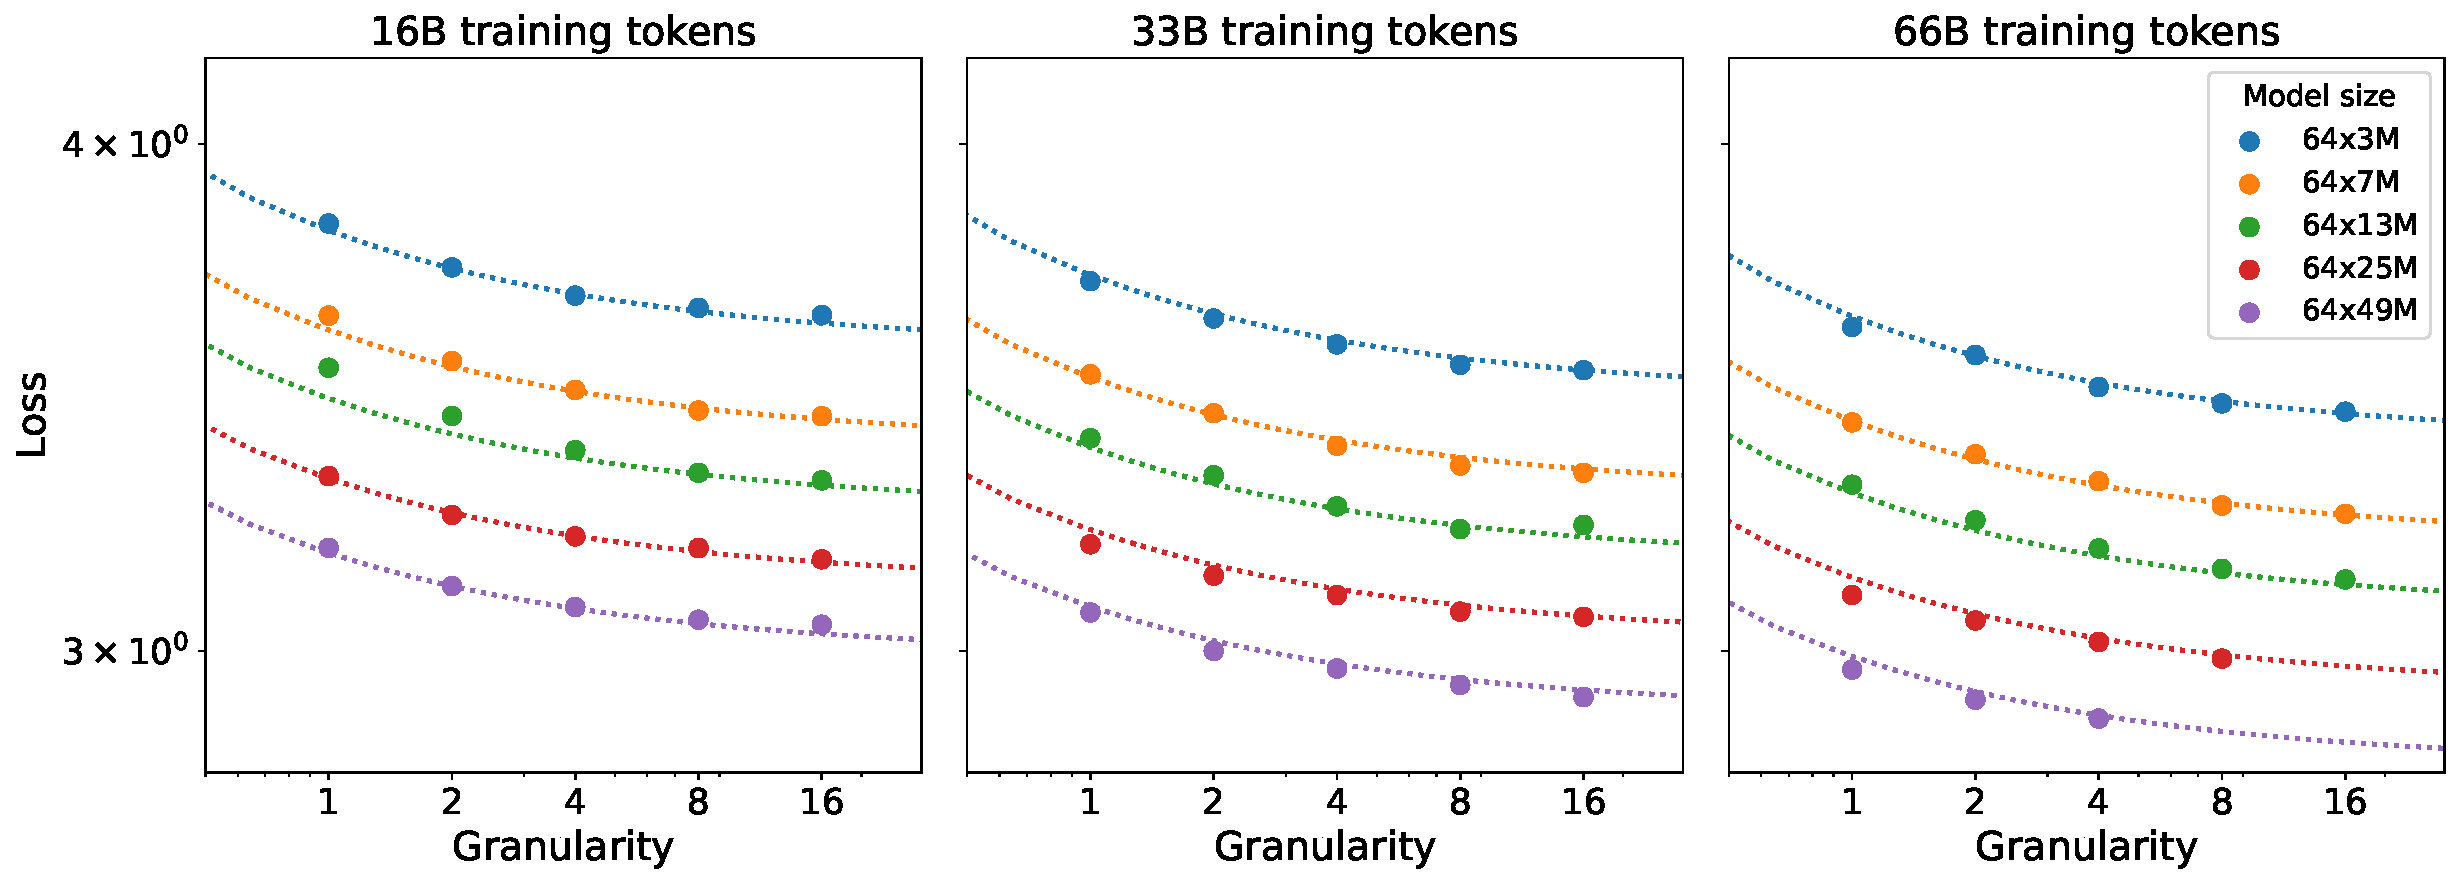
\includegraphics[width=.99\textwidth]{figures/final_fit_6.pdf}
  % \medskip
  \caption{Fit of the scaling laws compared to the experimental results.}
  \label{fig:scalinglaws}
\end{figure*}
Subsequently, we fit parameters in Eq. \ref{eq:loss_moe} to describe the scaling of MoE. For comparison, we also perform fitting for dense transformer given by Eq.~\ref{eq:chinchilla}. Similarly to \cite{hoffmann2022training}, we use Huber loss \citep{huber_loss}, with $\delta=0.1$. The optimization is performed using the BFGS algorithm. We include a weight decay of $5e-4$ to enhance generalization. We start with fitting parameters in Eq.~\ref{eq:loss_moe} and then find architecture-dependent coefficients $\alpha, \beta, A$ and $B$ in Eq.~\ref{eq:chinchilla}. We observe a good fit, with $\text{RMSE}=0.015$. The values are presented in Table \ref{tab:coeffs_scaling}. We depict the results in Figure~\ref{fig:scalinglaws}. 

\newpage
\subsection{Fitting the Parametric Scaling Law}\label{sub:parametric}
% \begin{align}\label{eq:loss_moe_num}
% \begin{split}
%     \mathcal{L}=
%     0.472 + \left(\frac{2.07}{G^{0.584}}+ 18.10\right)\frac{1}{N^{0.115}} + \frac{30.83}{D^{0.147}}.
% \end{split}
% \end{align}
\begingroup
\begin{table}[h]
    \centering
        \setlength{\tabcolsep}{5pt} 
    \caption{Values of the fitted coefficients.}
    \vspace{0.2cm}
    \begin{tabular}{ccccccccc}
        \toprule
        Model  & a & $\alpha$ & b & $\beta$ & g & $\gamma$ & c \\
        \midrule        
        MoE  & 18.1 & 0.115 & 30.8 & 0.147 & 2.1 & 0.58 & 0.47 \\ 
        Dense & 16.3 & 0.126 & 26.7 & 0.127 & - & - & 0.47\\
        \bottomrule
    \end{tabular}
    \label{tab:coeffs_scaling}
\end{table}
\endgroup

We validate the stability of the fit by excluding the top $20\%$ of models with the lowest perplexity and finding the coefficients based on the remaining experiments. We observe that the formula remains almost unchanged in this scenario (see Table \ref{tab:coeffs_valid} in Appendix \ref{app:coeffs_valid}). The validation RMSE is 0.019. Results are depicted in Figure~\ref{fig:valid_wall} (a).  

\begin{figure*}[t]
  \centering
  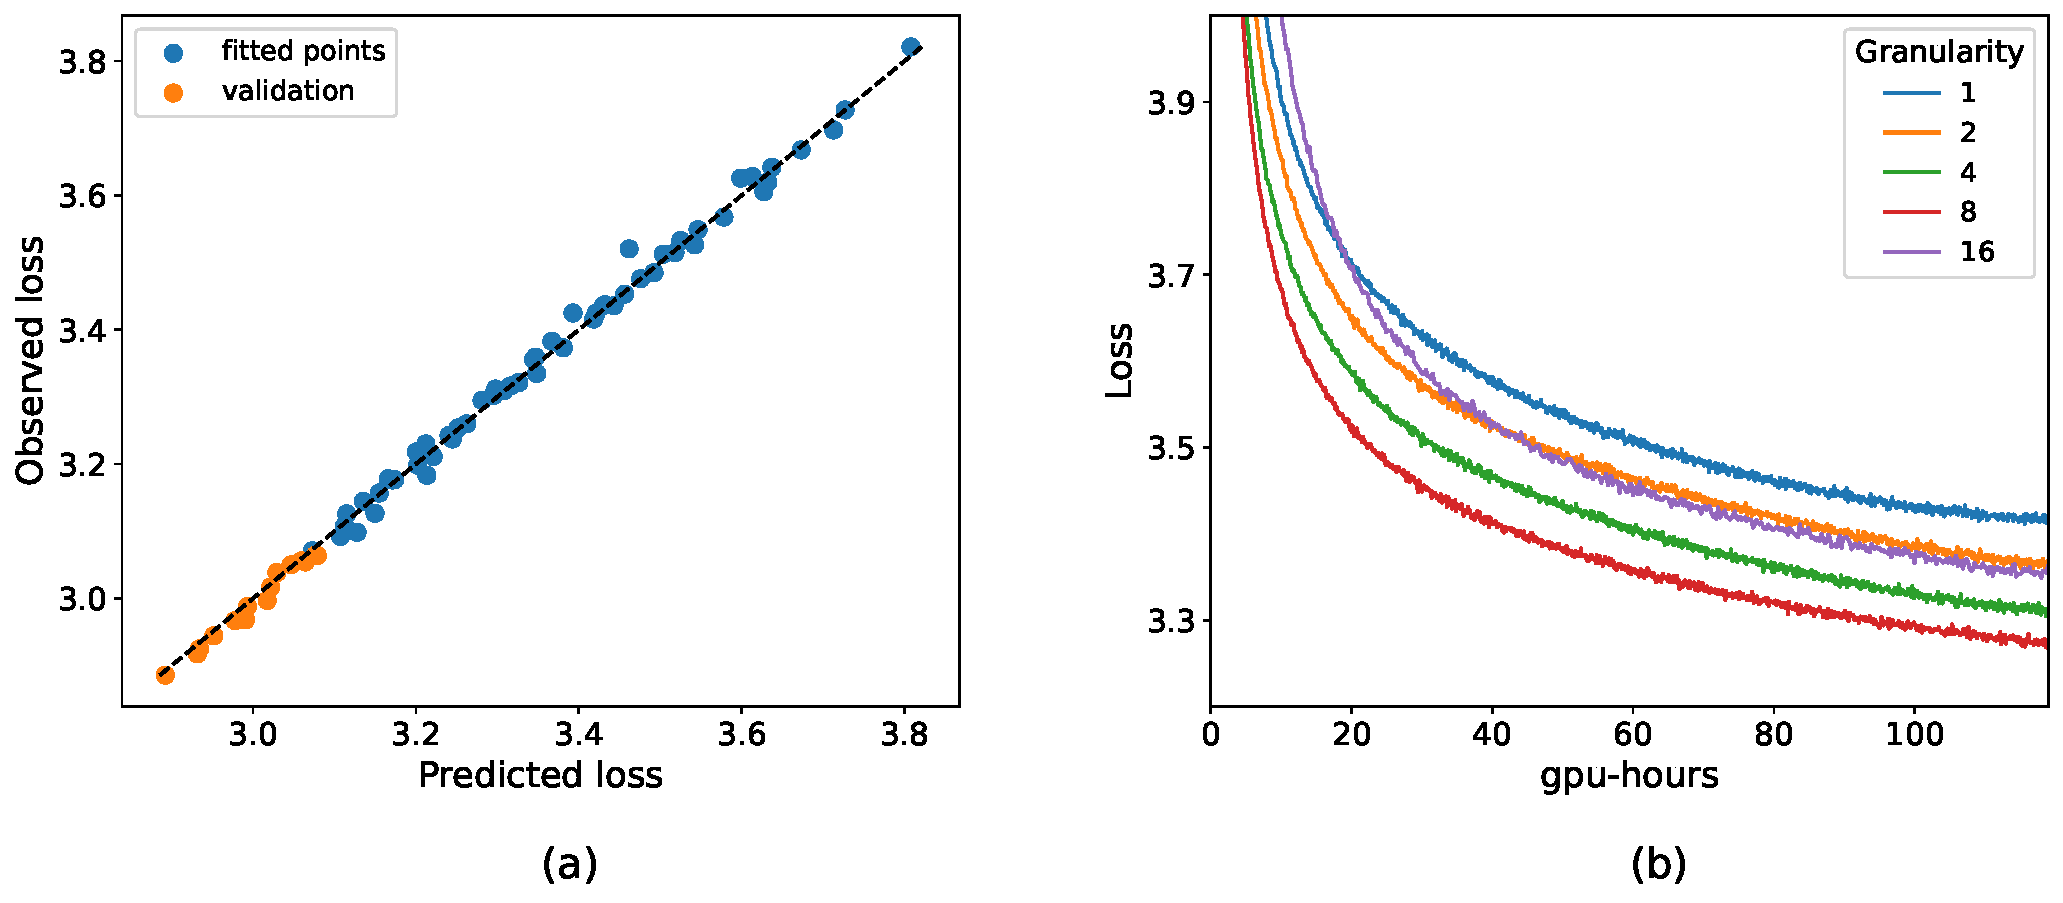
\includegraphics[width=.9\textwidth]{figures/valid_wall_clock.pdf}
  % \medskip
  \caption{\textbf{(a)} Validation of the scaling laws. \textbf{(b)} Training loss curves for model with $N=64 \times 7M$, $D=66B$ tokens, measured against wall-clock time on NVIDIA A100 GPU. $G=8$ leads to the best performance, as for $G=16$ the routing cost dominates gains from granularity. We model the increased cost of routing by measuring FLOPs for each configuration.}
  \label{fig:valid_wall}
\end{figure*}

% \begin{figure}[ht!] 
% \centering
% \includegraphics[width=0.45\textwidth]{icml2024/figures/validation.pdf}
% \caption{Validation of the fit.}
% \label{fig:validate}
% \end{figure}


\subsection{MoE Scaling Properties}\label{sub:scaling_properties}
%\ps{Ja nie rozumiem początku tego zdania.}
Comparing the part of the formula that approximates underfitting (that is, dependent on training tokens) in MoE ($30.8D^{-0.147}$) and Transformer ($26.7D^{-0.127}$), we can infer that MoE models need longer training to perform competitively but scale better after reaching that point. Nonetheless, this moment may still precede the compute optimal for both models.
%This is consistent with the common practice of longer training runs for sparse models present i.e in \cite{clark2022unified}. 
On the other hand, we can see that the exponent on dense models $\alpha=-0.126$ scales better with a total number of parameters than the MoE counterpart $\alpha=-0.115$. This should not be surprising since dense models use all parameters on each token contrary to MoE, which gains a computational advantage by activating only a subset of them. Therefore, the fair comparison of the performance has to take into account FLOPs used by each model type. In the next section, we find compute-optimal granularity for a given FLOP budget. 

% \jk{poprzednia wersja:}
% To fit this equation, similarly to \cite{hoffmann2022training}, we use BFGS algorithm working in log-scale. In order to compare our laws with baseline dense models, we also tune vanilla chinchilla scaling law within our training setup. However, for a fair comparison, both methods should have the same dataset bias $L_0$. Therefore we sweep over values from $(0,2)$ using intervals of $0.1$ and choose the value that gives us lowest approximation error for the fitted law, summed for both model classes. This also helps with the numerical stability of the approximation.
% Now we fit this equation and observe on figure \ref{fig:error} that this functional form allows for accurate prediction of the loss\jk{I would rather put the exact fitted values in the table} \sj{Maybe in the table as well, but I really like to see equation as a whole. Provides intuition, and it'll sell.}:

% \begin{align*}
%     L_f(N,D,G) = 0.5 + (5.52G^{-0.11}+{12.2})N^{-0.10} \\
%     + {485}D^{-0.28}
% \end{align*}
% \ps{tutaj brakuje jakiejś analizy błędów, np. 10 i 90 centyl}
% \subsection{Analysis of the Fitted Equation}\label{sub:analysis}
% \jk{Zakomentowałem część, która już jest w poprzednim fragmencie}
% % These parameters show, that granularity does not have interaction with training steps, however the interaction with number of parameters $N$ is significant and is the one responsive for the better performance of granular models. Therefore, we can reduce our scaling law to:
% % \begin{align*}
% %     L_s(N,D,G) = 0.5 + (2G^{-0.53}+{16.4})N^{-0.1} + 504D^{-0.28}
% % \end{align*}

% % \mk{to chyba jest do poprzedniego zdania, więc 'while'?} While the baseline fitted to $ 0.5 + 17.9N^{-0.14} + 30D^{-0.12}$. 
% Since in dense models, the tokens underfitting approximation is $30D^{-0.12}$, comparing to $504D^{-0.28}$ we can infer, that MoE models need longer training to perform competitively, but scale better after reaching that point. On the other hand, we can see that the exponent on dense models $N^{-0.14}$ scales better with number of parameters than the MoE counterpart $N^{-0.1}$. This should not be surprising, since dense models use all parameters on each token contrary to MoE, which  gain advantage by using computational power more efficiently. Therefore, final assessment of the performance has to take into account FLOPs used by each type of model.

% \jk{Na razie zakomentowuję quality of the fit. Ta informacja jest zawarta już na obrazku "Fit of the scaling law compared to experimental results". Dodatkowo myślę że damy osobny wykres "quality of the fit" z walidacją.}
% \begin{figure}[ht]
% \centering
% \includegraphics[width=0.4\textwidth]{icml2024/figures/error.png}
% \caption{Quality of the fit (MSE=0.0011). Similarity to \cite{hoffmann2022training}, error is higher on smaller models due to use of Huber loss, but prediction is not biased by granularity. \sj{Apart from the chart, it would be convincing to get some numbers - e.g. average bias/residual for each granularity; percent of variance unexplained by our scaling law, etc.} \janek{tutaj chyba lepszym argumentem, ze dziala i nie jest biased by granularity jest ten wykres \ref{fig:line}}}
% \label{fig:error}
% \end{figure}


%\begin{figure*}[ht]
%\centering
%\includegraphics[width=1.0\textwidth]{icml2024/figures/noline.png}
%\caption{A picture like that will be here. Caption: We verify our scaling results on the 3B scale. The model is }
%\label{fig:no_line}
%\end{figure*}

% \begin{figure*}[ht]
% \centering
% \includegraphics[width=0.7\textwidth]{icml2024/figures/intuition.png}
% \caption{(Left): Varying. (Right): ...}
% \label{fig:intuition}
% \end{figure*}

% \begin{figure*}[ht]
% \centering
% \includegraphics[width=1.0\textwidth]{icml2024/figures/gran_linear.png}
% \caption{Verification of our unified scaling laws for different training hyper-parameters. Granularity seem to not bias our loss predictions. \janek{tutaj musimy wstawic wykres faktycznej weryfikacji} }
% \label{fig:line}
% \end{figure*}

%\begin{figure}[ht]
%\centering
%\includegraphics[width=0.5\textwidth]{icml2024/figures/predict_scaling.png}
%\caption{A picture like that will be here. Caption: We verify our scaling results on the 3B scale. The model is }
%\label{fig:two_times}
%\end{figure}


\section{Optimal Allocation of Computational Budget }\label{sec:scaling_app}
%\subsection{Optimal Allocation of the Computational Budget}

In Section \ref{sec:scaling_laws}, we show that higher granularity leads to lower loss for the same number of training steps. This is not always the case if we consider the wall-clock time. As depicted in Figure \ref{fig:valid_wall} (b), in practice for too high values of $G$ (relative to $\dmodel$), training can be bottlenecked by the routing cost. Practical modeling of this situation is possible by measuring FLOPs in routing.
In this section we find optimal $N,D,G$ for a given computational budget $F$ 
% As seen in Figure \ref{fig:valid_wall} (b), \jk{dodać odniesienie do wall-clock time} 
% This can be done 
by solving the following optimization problem,
\begin{equation*}
    \begin{aligned}
        & \underset{N, D, G}{\text{minimize}}
        & & \mathcal{L}(N, D, G) \\
        & \text{subject to}
        & & \text{FLOPs}(N, D, G) = F.
    \end{aligned}
\end{equation*}


\subsection{Computational Cost of Granularity} \label{sub:compute_optimal}

%As we consider granularity in MoE models, 

It is important to acknowledge that increasing granularity can lead to some challenges in training the model, namely higher computational and communication costs and a larger memory footprint. The main component responsible for higher costs is the increase in routing operations due to a larger pool of granular experts. This increase is proportional to the value of $G.$ For standard, non-granular MoE models ($G=1$), the routing overhead still exists, although it has been considered negligible. 
%Nonetheless, the routing cost increases linearly with granularity. 
%for some smaller models it can become a bottleneck. 
%Then the number of FLOPs is solely determined by the number of parameters, that is $F=6N$ \cite{hoffmann2022training}, and is independent on other transformer parameters such as $\dmodel$ and the number of blocks, $\nblocks$. 

%In the case when $G > 1$, the computational budget should include both the cost of MoE layers and routing operations. 
% We would like to emphasise that all of these factors are dependent on the infrastructural details of the training. However, in order to realistically model these difficulties, in this section we would like to model the practical cost of increasing granularity.
 % Then 
Taking into account the routing operation overhead, the number of used FLOPs $F$ is described by the following formula:
\begin{align}
    F = (12{\dmodel}^2c_f + \dmodel EGc_r) \cdot D \cdot \nblocks,
    \label{eq:flops}
\end{align}
given expansion rate $E$, granularity $G$, and constants that denote FLOPs per active parameter ratio, respectively, within routing ($c_r$) and within the rest of the network ($c_f$). The term $12{d_{\text{model}}}^2$ is the number of active parameters within a transformer block, while $d_{\text{model}}EGc_r$ is the number of active parameters within a routing network. The in-depth analysis of constants $c_r$ and $c_f$ can be found in Appendix
\ref{app:constants}. We exclude embedding and unembedding from the FLOPs calculations, following \cite{hoffmann2022training}.

Observe that, in contrast to scenarios where routing operations are omitted, the FLOPs calculation that incorporates routing overhead relies on both $d_{\text{model}}$ and $\nblocks$. Consequently, an additional condition is required to determine the scaling of $d_{\text{model}}$ and $\nblocks$ in relation to an increase in $N$, the number of parameters. It is noted that minor variations in the depth-to-width ratio are not significant \citep{kaplan2020scaling}. Following this analysis, we opt to adopt the assumption that $\dmodel=64\nblocks$.

The total number of parameters in the feed-forward layer, excluding the routing matrix, is $2E\dff d_{\text{model}} = 8E{\dmodel}^2$, and $4{\dmodel}^2$ in attention (key, query, value, and output projection). This results in the following formula for the total number of parameters, $N = {\dmodel}^2 \cdot (8E + 4) \cdot \nblocks$.



%the same as in the standard transformer, the total number of non-embedding parameters in our feed-forward layer


%\sj{what is E? this is not mentioned. Also what about attention? $c_f=4$ seems bullshit , we need also some const like $4/8$ for dff and two FF matrices. $FF=8*dmodel^2$ (*6 to get flops) params. $routing=dmodel*E*G params$ (*6 to get flops), and also $dmodel*E*G*2(or 4)$ for routing, attention $is dmodel^2*4$ params (*6 to get flops), and we discount attention mechanism itself, or we can assume $dmodel=seq_len$ or something and get s$eqlen*dmodel*2$ (or 4, idk)} 

% In sum, given $N, D, G$, we infer the transformer model architecture parameters by solving the following system of equations,

% \begin{align*}
% F = (12{\dmodel}^2c_f + \dmodel EGc_r) \cdot \ntokens \cdot \nblocks\\
%  N = d_{\text{model}}^2 \cdot (8E + 4) \cdot n_{\text{layers}}, \\
%  d_{\text{model}} = 64 \cdot n_{\text{layers}}
% \end{align*}

% As a result, the optimization problem becomes, given a fixed number of floating-point operations (FLOPs) $F$,


\subsection{Compute Optimal Formula} \label{optimi}

Taking into consideration we need to solve the following optimization problem, given $F$,

\begin{equation*}
    \begin{aligned}
        & \underset{N, D, G}{\text{minimize}}
        & & \mathcal{L}(N, D, G) \\
        & \text{subject to}
        & & F = (12{\dmodel}^2c_f + \dmodel EGc_r) \cdot D \cdot \nblocks\\
        & & & N = d_{\text{model}}^2 \cdot (8E + 4) \cdot n_{\text{layers}}, \\
        & & & d_{\text{model}} = 64 \cdot n_{\text{layers}}.
    \end{aligned}
\end{equation*}

All these constraints are reducible to a one-dimensional optimization problem, which is, however, hard to solve analytically. Therefore we approximate the solution using Brent's method \citep{Brent1971AnAW}. The results of this optimization for varying FLOPs budgets are plotted in Figure \ref{flag_plots} while the optimal configurations of parameters for selected model sizes are presented in Table \ref{compute_opt}. To validate the uncertainty of these predictions, we follow \cite{hoffmann2022training} and calculate the 10$\text{th}$ and 90$\text{th}$ percentiles estimated via bootstrapping data (see Appendix \ref{app:reliabiliy} for the detailed results).
%\jk{continue here}
%We validate reliability of these constants in Appendix \ref{app:reliabiliy}.

\begin{table}[h]
    \centering
    \caption{Compute optimal training hyper-parameters for MoE models. Optimal $N$ and $D$ follow approximately similar relation to these of \cite{hoffmann2022training} for active parameters around the range of $1B$ to $10B$ parameters, requiring comparably longer training for smaller models and shorter for bigger ones. Higher granularity is optimal for larger compute budgets.
    % Note that, this also considers optimal granularity and its FLOPs cost.  
    }
    \vspace{0.2cm}
    \begin{tabular}{ccccc}
    \toprule
        N & D & G & FLOPs & Loss \\
        \midrule
        64 x 100M & 4.37B  & 8 & 2.95e+18 & 3.133 \\ 
        64 x 1B & 28.94B  & 16 & 1.93e+20 & 2.491 \\
        64 x 3B & 72.90B  & 16 & 1.41e+21 & 2.245\\
        64 x 7B & 137.60B  & 32 & 6.46e+21 & 2.076 \\
        64 x 70B & 941.07B  & 32 & 4.16e+23 & 1.694  \\
        64 x 300B & 2.96T & 64 & 5.69e+24 & 1.503  \\
        64 x 1T & 7.94T  & 64 & 4.97e+25 & 1.367 \\
        \bottomrule
    \end{tabular}
    % and we can observe, that increased granularity results in shorter compute optimal training.
    \label{compute_opt}
\end{table}





%\sj{I'd provide some examples of medium- and large-scale models that roughly follow this ratio (and if they don't, it's sus).} \janek{chinchilla ma 8.192/80=102.4, w kaplan scaling maja tam w "3 Empirical Results and Basic Power Laws" ablacje różnych depth to width ratio i mówią, że od nwm na oko 32 do 128 (to jest na wykresie) performance jest taki sam mniejwięcej i to mało zmienia, można jakoś dokładnie zaznaczyć to odwołanie. Poza tym nasze configi tak mają mniejwięcej też, co myśle, że dawałoby jakiś bias jakby założenie nie było zgodne z configami}.  


% Thus, to find optimal $N,D,G$, we need to solve a given constrained parameterized optimization problem:

%  {\it Given $F$, solve:}
% \begin{align*}
%     \argmin_{N,D,G} L_s(N,D,G)  
% \end{align*}
% {\it under constraints: }
% \begin{align}
%     \text{FLOPs}(n_{model}, E, \nblocks, G, D)=F  \\
%      N = {\dmodel}^2 \cdot (8E + 4) \cdot \nblocks \\
%      \dmodel=64 \cdot \nblocks 
% \end{align}

% \marekc{I suggest the following refomulation, which I consider more standard in terms of defining an optimization problem.}



% TODO check that params formula
%All these constraints are reducible, however the remaining optimization problem remains hard to solve analytically, therefore 



% \begin{figure}[ht!]
% \includegraphics[width=0.47\textwidth]{icml2024/figures/flops_compare.png}
% \caption{
% Relative number of FLOPS needed to train Transformer and Vanilla MoE (MoE with $G=1$) to achieve the performance of Granular MoE (MoE with compute optimal $G$). All curves assume selecting compute optimal $\nparams$ and $n_{tokens}$ for given FLOPS budget.}
% \label{fig:flops_save}
% \end{figure}




\subsection{MoE is Always More Efficient} \label{moe_more_eff}
Contrary to the results from \cite{clark2022unified}, in Figure \ref{flag_plots} we can see, that Mixture-of-Experts can be always considered more efficient than dense Transformers, regardless of the model size. According to our previous observations from Section~\ref{sub:scaling_properties}, MoE models scale better with optimal training. However, for short training schedules, they may under-perform dense models. This means that for constant training time and increasing model size, there exists a point where both models will become very under-trained, in which scenario dense models surpass MoE. This shows why in \cite{clark2022unified}, where varying the number of training tokens has not been considered, MoE was predicted to be under-performing for models bigger than $1T$. However, when all training hyper-parameters $N,D,G$ are properly selected to be compute-optimal for each model, the gap between dense and sparse models only increases as we scale.

%, what can be represented using our scaling laws as $ \forall_{c_g>0} \exists_{N>0} c_gN^{-0.10} > 17.9N^{-0.14}$

%\subsection{Optimal allocation of the compute budget}
%\begin{figure}[ht!]
%\centering
%\includegraphics[width=0.5\textwidth]{icml2024/figures/optimal_compute.png}
%\caption{Optimal allocation of the compute budget}
%\label{fig:compute}
%\end{figure}

\section{Discussion}\label{sec:analysis}
% \subsection{Training setup}\label{sub:setup}
% Why we used expert choice, specific models etc.

% \subsection{Autoregressive Expert Choice}
% Other interesting results: expert choice for autoregressive models (group size matters); expert choice evaluated as token choice; results for varying expansion rate. Our Granular MoE, in contrast to regular Expert Choice can be used on each layer, bringing in consistently to the architecture.

% \subsection{Fine-Tuning Expert Choice as Token Choice}
% In our experiments we explored the impact of routing strategies on model performance. Initially employing standard expert-choice routing, where each expert chooses some number of tokens from each position in sequence from fraction of batches, independently for each position in sequence, we observed a significant decrease in model performance when transitioning to token-choice routing, where each token determines the fraction of experts it attends to, while keeping all weights unchanged.

% To address the performance decline in token-choice routing, we fine-tuned the model trained with expert-choice routing to token-choice routing without introducing additional balancing loss, a typical component countering routing imbalance \cite{shazeer2017outrageously, fedus2022switch}. Remarkably, the fine-tuned model, rapidly rebounded to a perplexity level comparable to that of expert choice, highlighting the adaptability of the MoE architecture.

% These results hold promise, particularly since evaluating as an expert-choice requires a large batch, a constraint that is not universally applicable. In contrast, token-choice routing proves to be batch-size independent and, given its comparable effectiveness to expert choice, emerges as a superior alternative at inference.
% \sj{Include, somewhere, "There is a need to include transfer costs, and not only FLOPs, in Scaling Laws, especially with MoE. While this is extremely hardware dependent, and still number of FLOPs.}
% \jk{dodać jakiś wykresik że nasze predykcje korespondują z czasem. To widać np. na medium z }
% \jk{dodaję Future Work do tytułu, można to usunąć. Ale wydaje mi się że w dużym stopniu mamy tu Future Work}


\paragraph{Extreme Granularity.}
In Section \ref{sec:scaling_laws}, we argue that model performance improves with increasing granularity. This postulate largely aligns with the empirical findings of our study. Nonetheless, at exceedingly high granularity levels, such as $G=64$ in models characterized by $\dmodel=256$  and $E=64$, there is an observable decline in performance. This phenomenon is particularly evident in scenarios where the number of parameters in the routing mechanism exceeds active parameters in actual experts. Additionally, as described in Section \ref{sec:scaling_app}, the utility of such high granularity is predominantly restricted to models of substantial size. In alignment with the principles outlined by \cite{hoffmann2022training}, this research focuses more on findings that can be broadly applied rather than delving into the specific details of these corner-case situations. However, it is hypothesized that the efficiency of models with significantly high granularity could be potentially enhanced through careful expert initialization or modifications to the routing algorithm. These ideas are set aside to be investigated in future studies.

\paragraph{Varying Expansion Rate.}
In this study, due to computational resources constraint, we focus on $E=64,$ as recommended by \cite{clark2022unified}. This value of $E$ was also used for the largest models in other works \citep{du2022glam, zhou2022mixtureofexperts} and the best-performing configuration in \cite{fedus2022switch}. Nonetheless, we acknowledge the importance of considering different expansion rates, as different levels of $E$ may be chosen based on factors like the target size of the model in memory. Therefore, in Appendix~\ref{app:exp_rate}, we present the results of the study for $E=16$ and show that the main findings of this work are still valid in such cases. 
%The number of experiments needed to consider various values of expansion rate has made it practically infeasible for us, as we already model dataset size and granularity. 
%\janek{to jedno nastepne zdanie bym przerzucil juz do tego appenixu} In particular, higher granularity is more optimal when increasing the compute budget. We also observe that with $E=16$ MoE models always outperform dense Transformers, and that the gap widens with scale.

\paragraph{Including $E$ in the formula.} Another possible advancement would be to unify all of the factors $N, D, G$ and $E$ in one formula. While this would open the possibility of studying the relationships between coefficients in more detail, it would also be hard to practically recommend the optimal configuration in such a scenario using only FLOPs. This is because larger values of $E$ typically lead to better performance but also incur additional memory requirements. Therefore, the choice of expansion rate may be heavily dependent on the available hardware configuration. We leave a detailed study of these factors for future work.

% (tutaj opisujemy, że tak naprawde extreme granularity się wygina i nie wiemy czemu, ale jest to zawsze dalekie od optimum a nasze scaling laws opisuja tak jak wszystkie laws modele niezdegenerowane. Może to wynikać z tego że w pewnym poziomie liczba parametrów w routingu jest większa niż w FF i napewno nie chcemy do takiej sytuacji doprowadzać albo od potencjalnie innej inicjalizacji)

\paragraph{Modeling the cost of granularity.}
It is important to note that the exact estimation of the training cost of MoE models is dependent on the training setup, hardware, and implementation. Specifically, increasing G can lead to higher transfer costs, depending on the adopted model of distributed training. Therefore, the precise selection of hyperparameters should be made considering these factors. In this work, we model the cost of operations using FLOPs, which is common in the Scaling Laws literature \citep{kaplan2020scaling, hoffmann2022training, frantar2023scaling}. Additionally, we would like to note that in our setup, we observe significant gains of fine-grained MoE measured as wall-clock time needed to achieve given perplexity (see Fig. \ref{fig:valid_wall} (b) for an example).  

% \begin{figure}[ht!]
% \centering
% 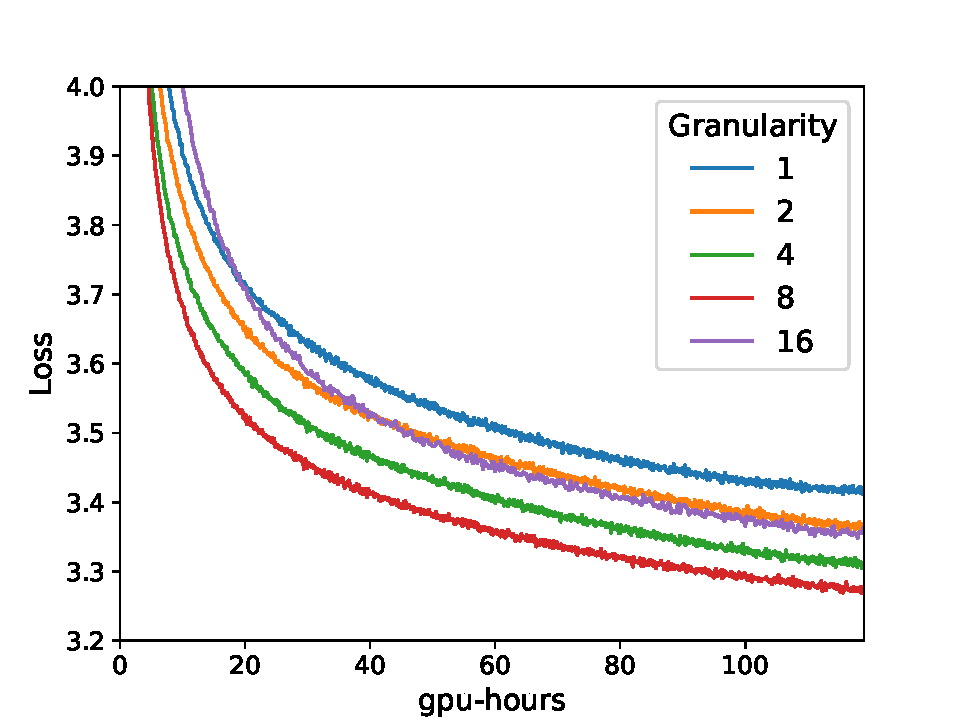
\includegraphics[width=0.6\textwidth]{figures/time.pdf}
% \caption{Training loss curves for model with $N=64 \times 7M$, $D=66B$ tokens, measured on NVIDIA A100 GPU. We can see that the model
% with $G=8$ achieves the best performance.}
% \label{fig:time}
% \end{figure}

% \jk{Jak zdążymy, dla uczciwości można coś dodać że te scaling laws moga być zależne od dokładnego setupu (typu tokenizer, dataset, itp. }

% \subsection{Larger Scale}
% In this study, we derive our conclusions based on over 100 experiments, spanning various parameters for dense and MoE models. While we are able to match the model sizes considered by \cite{kaplan2020scaling}, our compute capabilities are...
% W punktach, co tu ma być:
% 1. O ile rozważane przez nas wielkości modeli są porównywalne do tych używanych w [kaplan], nasze ograniczenia budżetu obliczeniowego są istotniejsze niż w przypadku 
% \jk{Tutaj jakaś obrona, dlaczego mamy takie wielkości modeli. Ze w sumie nasze modele są całkiem spore (total params), i że Kaplan też miał podobne. No ale że jakbyśmy mieli więcej compute, to byśmy dokładniej skalibrowali nasze wyniki. I że mimo wszystko nasze główne wnioski pozostają w mocy.}
% \jk{coś że nasze wyliczenia mogłyby być dokładniejsze}


\section{Conclusions}

This study introduces a novel hyperparameter, granularity ($G$), and underscores the significance of adjusting it for optimizing the efficiency of experts within MoE models.  A central finding of this research is that a standard granularity of $G=1$ is suboptimal across a broad range of FLOPs, leading to the recommendation of using higher granularity values to enhance MoE model performance and efficiency. Simultaneously, this work emphasizes the importance of varying training duration for compute-optimal settings. Consequently, both granularity and variable training length are incorporated into new scaling laws. These laws confidently demonstrate that MoE models consistently outperform dense transformers in terms of efficiency and scaling. This work not only sheds new light on the scaling laws applicable to MoE models but also provides practical guidance for improving computational efficiency in large language models. The insights are critical for the development and optimization of large-scale language models, marking a significant advancement in the field.


\section{Reproducibility}

The code used to produce the results described in this work is open-sourced and can be found at \href{https://github.com/llm-random/llm-random}{\texttt{github.com/llm-random/llm-random}}. 

\newpage
\section*{Acknowledgments}

We would like to express sincere gratitude to Piotr Miło\'s and Tomasz Trzci\'nski for valuable feedback and to Aleksandra Weglarz for her help with graphic design.

This work was funded by IDEAS NCBR, which also provided significant computational resources a supportive research environment and direction. The research was supported by PL-Grid infrastructure (grant PLG/2023/016148). We also benefited from the Entropy cluster (hosted at the Faculty of Mathematics, Informatics and Mechanics of the University of Warsaw) funded by NVIDIA, Intel, the Polish National Science Center grant 2022/45/N/ST6/02222, and ERC Starting Grant TOTAL. Marek Cygan was partially supported by an NCBiR grant POIR.01.01.01-00-0392/17-00.


% \newpage



\bibliography{iclr2024_conference}
\bibliographystyle{iclr2024_conference}

\appendix

%%%%%%%%%%%%%%%%%%%%%%%%%%%%%%%%%%%%%%%%%%%%%%%%%%%%%%%%%%%%%%%%%%%%%%%%%%%%%%%
%%%%%%%%%%%%%%%%%%%%%%%%%%%%%%%%%%%%%%%%%%%%%%%%%%%%%%%%%%%%%%%%%%%%%%%%%%%%%%%
% APPENDIX
%%%%%%%%%%%%%%%%%%%%%%%%%%%%%%%%%%%%%%%%%%%%%%%%%%%%%%%%%%%%%%%%%%%%%%%%%%%%%%%
%%%%%%%%%%%%%%%%%%%%%%%%%%%%%%%%%%%%%%%%%%%%%%%%%%%%%%%%%%%%%%%%%%%%%%%%%%%%%%%
\clearpage
\appendix
\onecolumn
\section{Architecture and Training Setup}\label{app:setup}
All of the models considered in this work are decoder-only Transformers trained on the C4 dataset \citep{raffel2023exploring}. We use GPT2 tokenizer \citep{radford2018improving}. Each batch consists of 0.5M tokens packed into 2048 sequences. Our optimizer is AdamW \citep{loshchilov2019decoupled}, with a weight decay of $0.1.$ In each training run, we use the maximum learning rate of $2\mathrm{e}{-4},$ with linear warmup for $1\%$ steps and cosine decay to $2\mathrm{e}{-5}.$ To improve stability, we initialize weights using the truncated normal distribution with reduced scale, as advised in \cite{fedus2022switch}. The models are trained using mixed precision; we always keep the attention mechanism and router in high precision. We assume the \textit{infinite data} regime, as the number of training tokens for any of the runs is less than the number of tokens in the corpus. We follow \cite{hoffmann2022training} and perform our analysis on the smoothed training loss.

In MoE, we use the Expert Choice routing algorithm, as it guarantees a balanced expert load without tuning additional hyperparameters. To maintain compatibility with autoregressive language modeling, we apply the recipe described in \cite{zhou2022mixtureofexperts}: tokens are grouped by position across different sequences. The group size is always set to $256.$ We match the number of FLOPs for MoE and dense models with the same $\dmodel$ (meaning we activate an average of $8\dmodel^2$ parameters per token in each MoE layer). In the router, softmax is performed over the expert dimension, while we choose tokens over the token dimension, as this leads to the best performance (as opposed to performing softmax over the token dimension). We put an additional layer normalization before the output of MoE layer. This gives a small improvement for standard MoE, but is crucial for the performance of models with $G>1.$

Table \ref{tab:moe} and Table \ref{tab:dense} list the considered architecture and training variants for dense and MoE models, respectively. 

\begin{table}[h] 
    \centering
    \caption{Architecture and training variants (MoE models).}
    \vspace{0.4cm}
    \begin{tabular}{ccccccc}
    \toprule
        \#parameters (nonemb) & $\dmodel$ & $\nblocks$ & $\nheads$ & $D$ (in \#tokens) & $G$\\
        \midrule
        64x3M  & 256 & 4 & 4 & 16B, 33B, 66B & 1, 2, 4, 8, 16  \\
        64x7M & 384 & 4 & 6 & 16B, 33B, 66B & 1, 2, 4, 8, 16 \\
        64x13M & 512 & 4 & 8 & 16B, 33B, 66B & 1, 2, 4, 8, 16 \\
        64x13M & 512 & 4 & 8 & 130B & 1, 2, 4 \\
        64x25M & 512 & 8 & 8 & 16B, 33B, & 1, 2, 4, 8, 16 \\
        64x25M & 512 & 8 & 8 & 66B & 1, 2, 4, 8 \\
        64x49M & 640 & 10 & 10 & 16B, 33B & 1, 2, 4, 8, 16 \\
        64x49M & 640 & 10 & 10 & 66B & 1, 2, 4 \\
        64x85M & 768 & 12 & 12 & 33B & 1, 2, 4 \\ \bottomrule
    \end{tabular}
    \label{tab:moe}
\end{table}


\begin{table}[h] \label{table_dense}
    \centering
    \caption{Architecture and training variants (dense models).}
    \vspace{0.4cm}
    \begin{tabular}{ccccccc}
    \toprule
        \#parameters (nonemb) & $\dmodel$ & $\nblocks$ & $\nheads$ & $D$ (in \#tokens) \\
        \midrule
        3M  & 256 & 4 & 4 & 16B, 24B, 33B, 66B \\
        6M & 256 & 8 & 4 & 16B, 24B, 33B, 66B \\
        13M & 512 & 4 & 8 & 16B, 24B, 33B, 66B \\
        25M & 512 & 8 & 8 & 16B, 24B, 33B, 66B \\
        49M & 640 & 10 & 10 & 16B, 24B, 33B, 66B \\
        85M & 768 & 12 & 12 & 16B, 33B \\
        \bottomrule
    \end{tabular}
    \label{tab:dense}
\end{table}

\newpage
\section{Validation of the Scaling Law}\label{app:coeffs_valid}
% In this section we list the best fit of coefficients in Eq.~\ref{eq:chinchilla} for dense models and Eq.~\ref{eq:loss_moe} for MoE models (see Sec. \ref{sub:joint}).
In this section, we provide coefficients of the scaling law fitted with 20$\%$ of datapoints with the lowest perplexity excluded for the purpose of validation.

\begin{table}[h]
    \centering
    \caption{Values of the fitted coefficients.}
    \vspace{0.4cm}
    \begin{tabular}{c|c|c|c|c|c|c|c|c}
        Model  & a & $\alpha$ & b & $\beta$ & g & $\gamma$ & c \\
        \hline
        MoE  & 17.6 & 0.114 & 26.7 & 0.140 & 2.07 & 0.570 & 0.472 \\ 
    \end{tabular}
    \label{tab:coeffs_valid}
\end{table}

\section{Reliability of Compute Optimal Formula}\label{app:reliabiliy}
In this section, we assess the stability of our predictions presented in Section~\ref{sub:compute_optimal}. Similarly to \cite{hoffmann2022training} we calculate the 10$^\text{th}$ and 90$^\text{th}$ percentiles estimated via bootstrapping data ($80\%$ of the data is sampled $100$ times). See Table \ref{tab:bootstrap} for the details.

\begin{table}[h]
    \centering
    \caption{10$^\text{th}$ and 90$^\text{th}$ percentiles estimated via bootstraping data.}
    \vspace{0.4cm}
    \begin{tabular}{ccc}
        \toprule
        N & D & G \\
        \midrule
        64 x 100M & (2.97B, 5.98B) & (8, 8) \\ 
        64 x 1B & (21.17B, 40.73B)  & (16, 16)  \\
        64 x 3B & (50.20B, 105.88B)  &  (16, 32)  \\
        64 x 7B & (101.06B, 205.40B)   &  (32, 32)  \\
        64 x 70B & (638.49B, 1.59T) & (32, 64) \\
        64 x 300B & (1.99T, 5.62T)  &  (64, 64) \\
        64 x 1T & (5.29T, 16.87T)   & (64, 64) \\
        \bottomrule
    \end{tabular}
    \label{tab:bootstrap}
\end{table}
\section{Varying Expansion Rate} \label{app:exp_rate}
In this section, we provide results for $E=16.$ The training procedure is the same as described in App. \ref{app:setup}. The models considered in this part are listed in Table \ref{tab:moe_16}. 

\begin{table}[h] 
    \centering
    \caption{Architecture and training variants (MoE models).}
    \vspace{0.4cm}
    \begin{tabular}{ccccccc}
        \toprule
        \#parameters (nonemb) & $\dmodel$ & $\nblocks$ & $\nheads$ & $D$ (in \#tokens) & $G$\\
        \midrule
        64x3M  & 256 & 4 & 4 & 8B, 16B, 33B & 1, 2, 4, 8, 16  \\
        64x7M & 256 & 8 & 4 & 8B, 16B, 33B & 1, 2, 4, 8, 16 \\
        64x13M & 512 & 4 & 8 & 8B, 16B, 33B & 1, 2, 4, 8, 16 \\
        64x13M & 512 & 4 & 8 & 66B & 1, 2, 4 \\
        64x25M & 512 & 8 & 8 & 8B, 16B, 33B & 1, 2, 4, 8, 16 \\
        64x49M & 640 & 10 & 10 & 8B & 1, 2, 4, 8, 16 \\
        \bottomrule
    \end{tabular}
    \label{tab:moe_16}
\end{table}

We fit Eq.~\ref{eq:loss_moe} using the same procedure as described in Section~\ref{sub:parametric}. The results are detailed in Table \ref{tab:_different_e}.

\begin{table}[ht!]
    \centering
        \caption{Values of the fitted coefficients.}
    \vspace{0.4cm}
    \begin{tabular}{ccccccccc}
    
    \toprule
        Model  & a & $\alpha$ & b & $\beta$ & g & $\gamma$ & c \\
        \midrule
        MoE ($E=16$)  & 19.64 & 0.124 & 57.07 & 0.169 & 1.18 & 0.986 & 0.472 \\  \bottomrule
    \end{tabular}
    \label{tab:_different_e}
\end{table}

Using the coefficients and FLOPs calculation formulas, we can derive the compute optimal training parameters. The results are presented in Table \ref{tab:compute_opt_16}.

\begin{table}[ht!]
    \caption{10$^\text{th}$ and 90$^\text{th}$ percentiles estimated via bootstrapping data for $E=16$.}
    \centering
    \vspace{0.4cm}
    \begin{tabular}{ccc}
    \toprule
        N & D & G \\
        \midrule
        16 x 100M & (10.29B, 17.73B)   & (8 , 16)  \\
        16 x 1B   & (53.74B, 103.54B)  & (16, 32)  \\
        16 x 3B   & (106.22B, 261.04B) & (16, 32)  \\
        16 x 7B   & (177.65B, 511.43B) & (16, 32)  \\
        16 x 70B  & (721.60B, 3.22T)   & (32, 64)  \\
        16 x 300B & (1.73T, 10.69T)    & (32, 64)  \\
        16 x 1T   & (3.60T, 28.22T)    & (32, 128)  \\ \bottomrule
    \end{tabular}
    \label{tab:compute_opt_16}
\end{table}

We can observe that similarly to the case when $E=64,$ larger compute budgets imply larger optimal values of $G.$ Note that the values for $10^\text{th}$ and $90^\text{th}$ percentiles form larger intervals in this case, as in this part we run a smaller number of experiments and keep shorter training durations. However, we believe that this preliminary study forms a valuable addition to the results in the main part.

% \section{Compute Optimal Granularity for Overtrained Models}

% \begin{table}[h]
%     \centering
%     \begin{tabular}{c|c|c|c|c|c}
%         N & D_{opt} & G_{opt} \text{ for } D_{opt} &  G_{opt} \text{ for } 2D_{opt} & G_{opt} \text{ for } 10D_{opt} & G_{opt} \text{ for } 100D_{opt}  \\
%         \hline
%         64 x 100M & 4.37B  & 8  & TBD & TBD & TBD  \\ 
%         64 x 1B & 28.94B  & 16  & TBD & TBD & TBD   \\
%         64 x 3B & 72.90B  & 16  & TBD & TBD & TBD   \\
%         64 x 7B & 137.60B  & 32  & TBD & TBD & TBD   \\
%         64 x 70B & 941.07B  & 32  & TBD & TBD & TBD  \\
%         64 x 300B & 2.96T & 64  & TBD & TBD & TBD   \\
%         64 x 1T & 7.94T  & 64  & TBD & TBD & TBD  \\
%     \end{tabular}
%     \caption{Compute optimal Granularity for overtrained models}
%     \label{tab:compute_opt_overtrained}
% \end{table}

% \janek{Moze dodac tabelke o tym jak dostosowywać granularity przy overtrained modelach, bo taka jest praktyka, zeby wyszlo taniej w inferencji? To brzmi jak dobry pomysl, zeby ludzie realnie tego uzywali.} 

%\section{Optimal Training Tokens for Different %Granularities}\label{app:copt_for_grans}

%\begin{table}[h]
    %\centering
    %\begin{tabular}{c|c|c|c|c|c|c|c}
        %N & D_{opt} & G_{opt} & D_{opt} \text{ for } G=1 & D_{opt} \text{ for } G=2 & D_{opt} \text{ for } G=4 & D_{opt} \text{ for } G=8  & D_{opt} \text{ for } G=16 \\
        %\hline
        %64 x 200M & 8.33B & 4 & TBD & TBD & TBD & TBD & TBD  \\ 
        %64 x 1B & 20.5B & 8 & TBD & TBD & TBD & TBD & TBD \\
        %64 x 3B & 58.1B & 8 & TBD & TBD & TBD & TBD & TBD \\
        %64 x 7B & 118B & 8 & TBD & TBD & TBD & TBD & TBD  \\
        %64 x 70B & 802B & 16  & TBD & TBD & TBD & TBD & TBD  \\
        %64 x 500B & 4.27T & 16 & TBD & TBD & TBD & TBD & TBD \\
        %64 x 1T & 7.76T & 16 & TBD & TBD & TBD & TBD & TBD  \\
    %\end{tabular}
    %\caption{Compute optimal training time for %different Granularities}
    %\label{tab:compute_opt_overtrained}
%\end{table}

%\janek{Dodatkowo można też dodać jakie są compute optimal dlugoscitreningu przy konkretnym granularity, jak to sie zmienia. Mysle, ze bedzie z tego wynikac, ze MoE sie trenuje dluzej dlatego, ze G=1, dla bardziej granularnych, w szcegolnosci takich z $G_{opt}$ trening zbiega do okolo chinchilli}
% \newpage
\section{FLOPs Constants}\label{app:constants}

The number of FLOPs $F$ used in Transformer training, considering the routing operation overhead in MoE, can be described by the following formula:
\begin{align}
     F = (12{\dmodel}^2c_f + \dmodel EGc_r) \cdot \ntokens \cdot \nlayers
    \label{eq:flops_overhead}
\end{align}

Following \cite{hoffmann2022training}, we assume $c_f$ to be $6$. This is interpreted as 6 FLOPs for each pair of an active parameter (in linear projection) and a processed token. The breakdown of operations is as follows:
\begin{itemize}
    \item During the forward pass, 2 operations (single multiplication and single addition) are used to compute the matrix multiplication of an input and linear projection.
    \item During the backward pass, 2 operations are used to compute gradients wrt. the input.
    \item During the backward pass, 2 operations are used to compute gradients wrt. the weights of linear projection.
\end{itemize}

In our work, we have assumed the routing constant, $c_r$, to be 14, with the breakdown presented below. The exact number of operations may depend on the implementation of routing, but it will be between 6 and 20. However, our main conclusions of the paper are resistant to different assumptions of this constant.
\begin{itemize}
    \item During the forward pass, 2 operations are used to compute the expert logits based on an input and ``routing linear projection''.
    \item During the backward pass, 2 operations are used to compute gradients for ``routing linear projection'' wrt. the input.
    \item During the backward pass, 2 operations are used to compute gradients for ``routing linear projection'' wrt. the weights of linear projection.
    \item During the forward pass, 2 operations are used to route input tokens to chosen experts.
    \item During the forward pass, 2 operations are used to route expert outputs to chosen tokens and multiply those outputs by the routing score.
    \item During the backward pass, 2 operations are used to route gradients from output tokens to experts.
    \item During the backward pass, 2 operations are used to route gradients from experts to input tokens.
\end{itemize}

Similarly to the calculation of FLOPs for $c_f$, FLOPs come in pairs as each multiplication is followed by an addition (used to accumulate outputs or gradients).

%We are aware that values of constants $c_r$ and $c_f$, and especially their capability to model actual time, are highly dependent on implementation, hardware and training environment. Therefore we think, that exact values should be fitted for specific training setup. Following \cite{hoffmann2022training}, we assume $c_f$ to be $6$. \janek{TODO, argumentować wybór cr na 14 na podstawie faktycznych flopsów}
% \newpage
% \section{Measuring Wall-clock Time}\label{app:time}
% In this section, we provide an example of training curves for models with different levels of granularity, measured in terms of wall-clock training time on NVIDIA A100 GPU. We can see that the model with $G=8$ achieves the best performance in this case.
% \begin{figure}[ht!]
% \centering
% 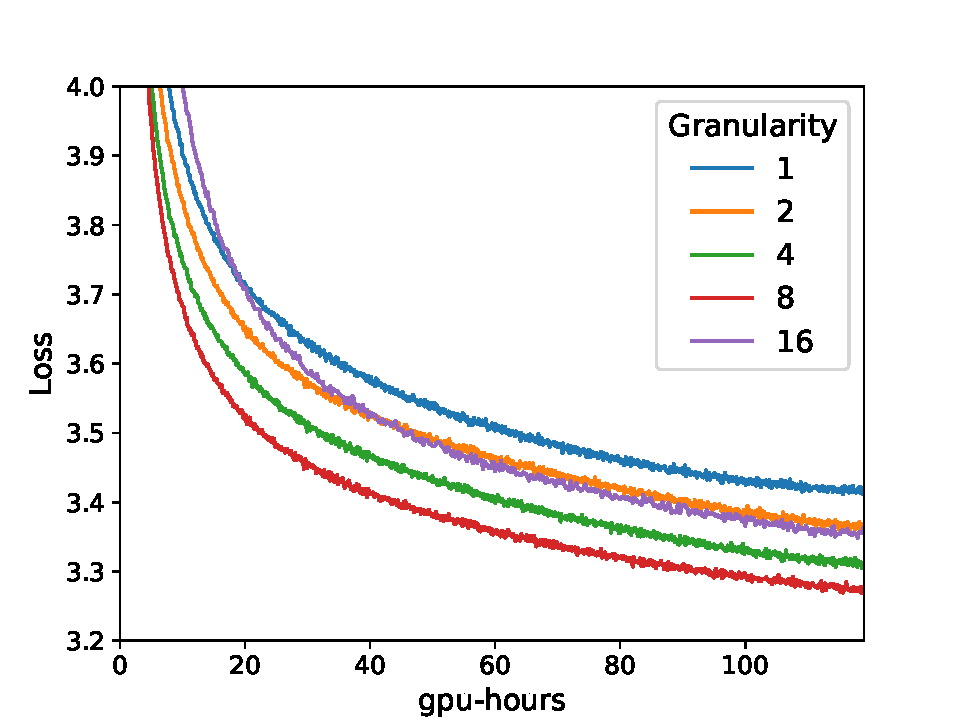
\includegraphics[width=0.6\textwidth]{figures/time.pdf}
% \caption{Training loss curves for model with $N=64 \times 7M$, $D=66B$ tokens.}
% \label{fig:time}
% \end{figure}
% \newpage
\section{Additional Visualizations}
\label{sec:app_add_viz}

\begin{figure}[ht!]
  \centering
  \begin{tabular}{ c @{\hspace{30pt}} c }
    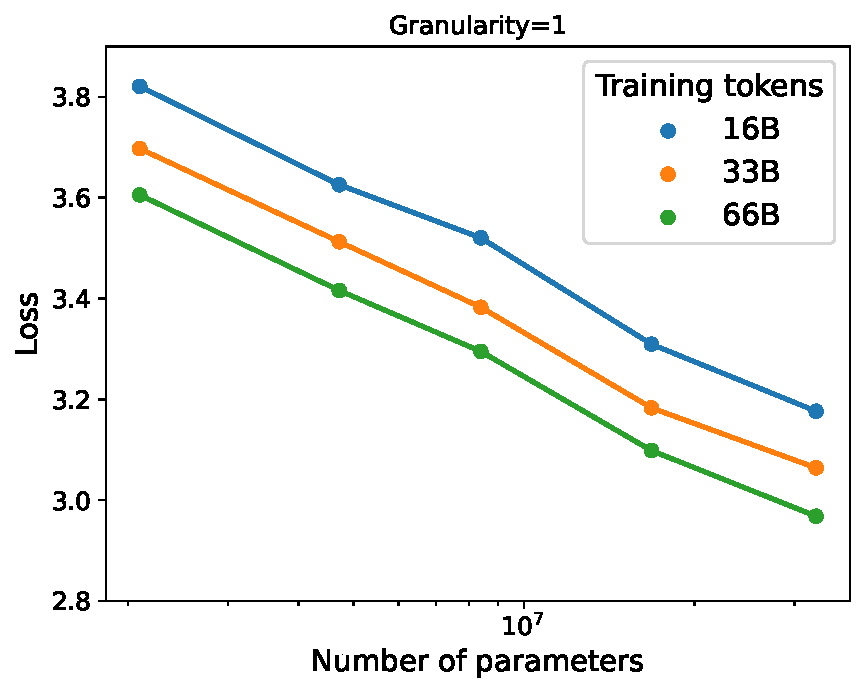
\includegraphics[width=.3\textwidth]{figures/kaplan_1.pdf} &
      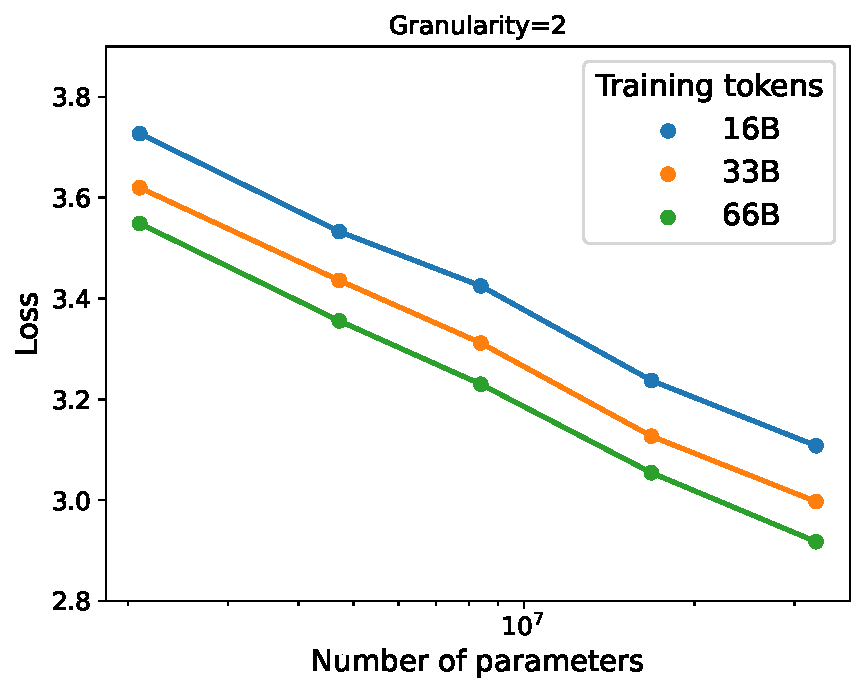
\includegraphics[width=.3\textwidth]{figures/kaplan_2.pdf} \\
    \small \textbf{(a)} &
      \small \textbf{(b)} \\
  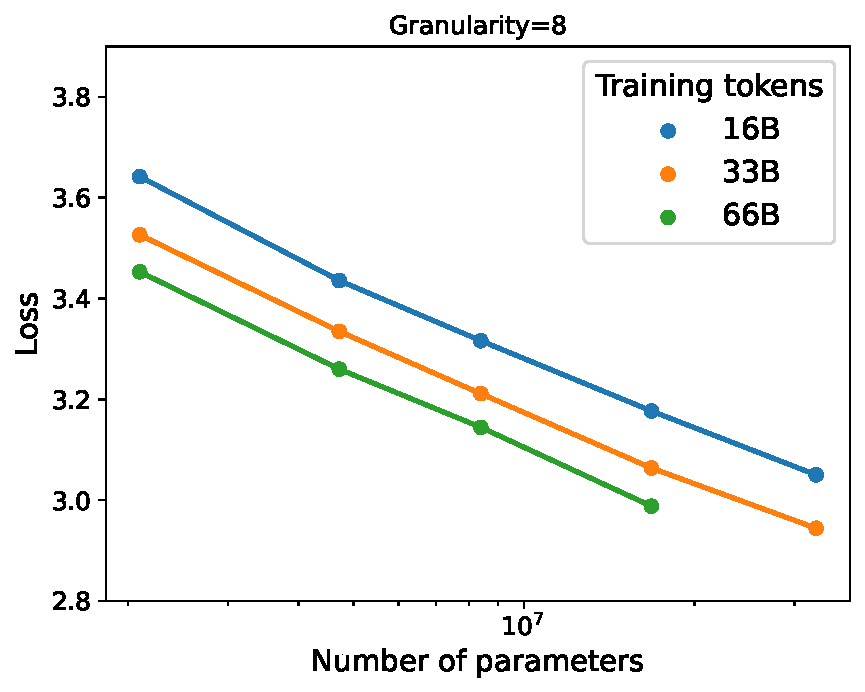
\includegraphics[width=.3\textwidth]{figures/kaplan_8.pdf} &
      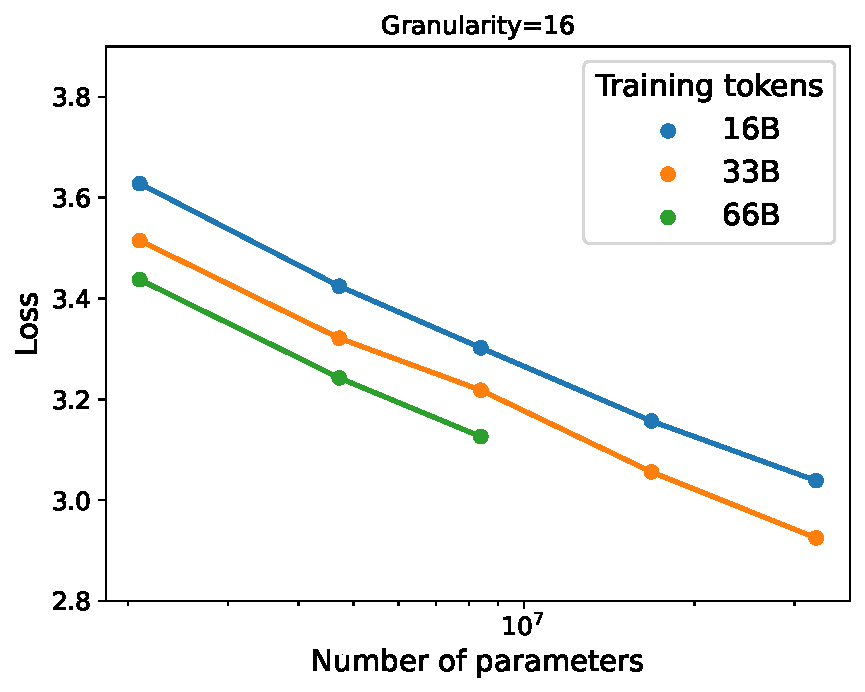
\includegraphics[width=.3\textwidth]{figures/kaplan_16.pdf} \\
    \small \textbf{(c)} &
      \small \textbf{(d)}
  \end{tabular}

  \medskip

  \caption{Illustration of scaling $N$ and $D$ for constant granularity value of: \textbf{(a)} $G=1$ \textbf{(b)} $G=2$ \textbf{(c)} $G=8$ \textbf{(d)} $G=16.$ }
  \label{line_gran_plot}
\end{figure}

\begin{figure}[ht!]
  \centering
  \begin{tabular}{ c @{\hspace{30pt}} c }
    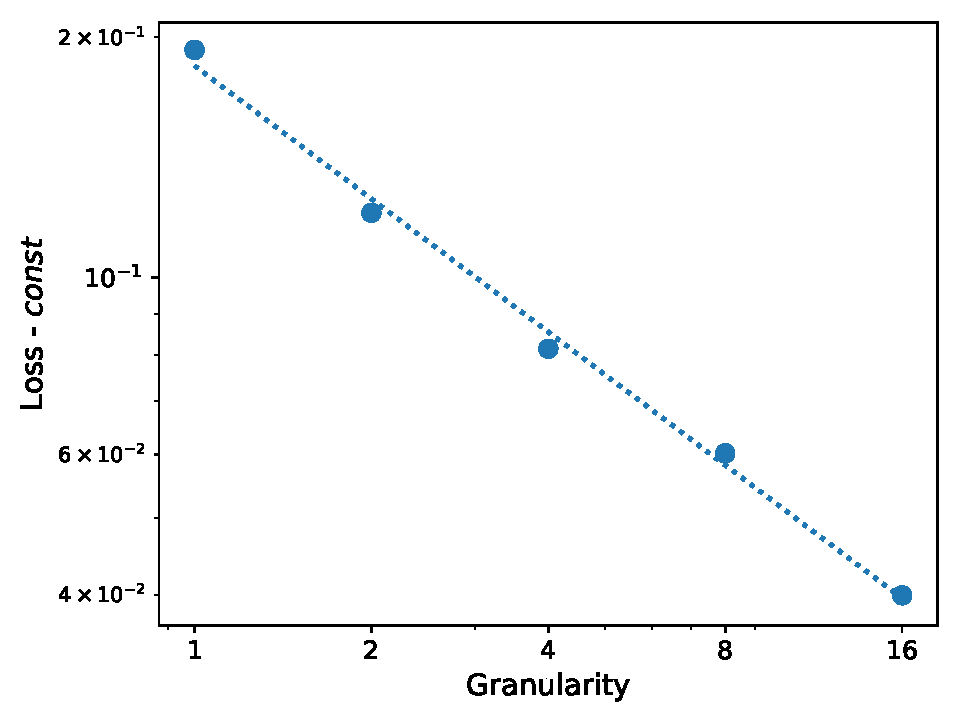
\includegraphics[width=.3\textwidth]{figures/granularity_N_1082130432_D_31250.0.pdf} &
      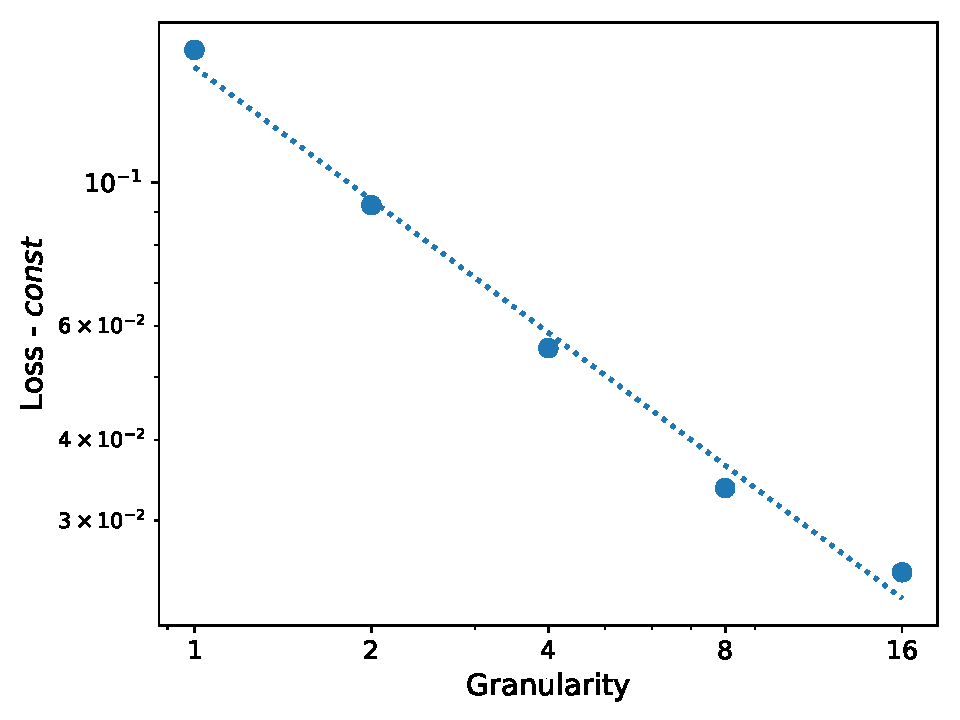
\includegraphics[width=.3\textwidth]{figures/granularity_N_2113536000_D_31250.0.pdf} \\
    \small \textbf{(a)} &
      \small \textbf{(b)} \\
  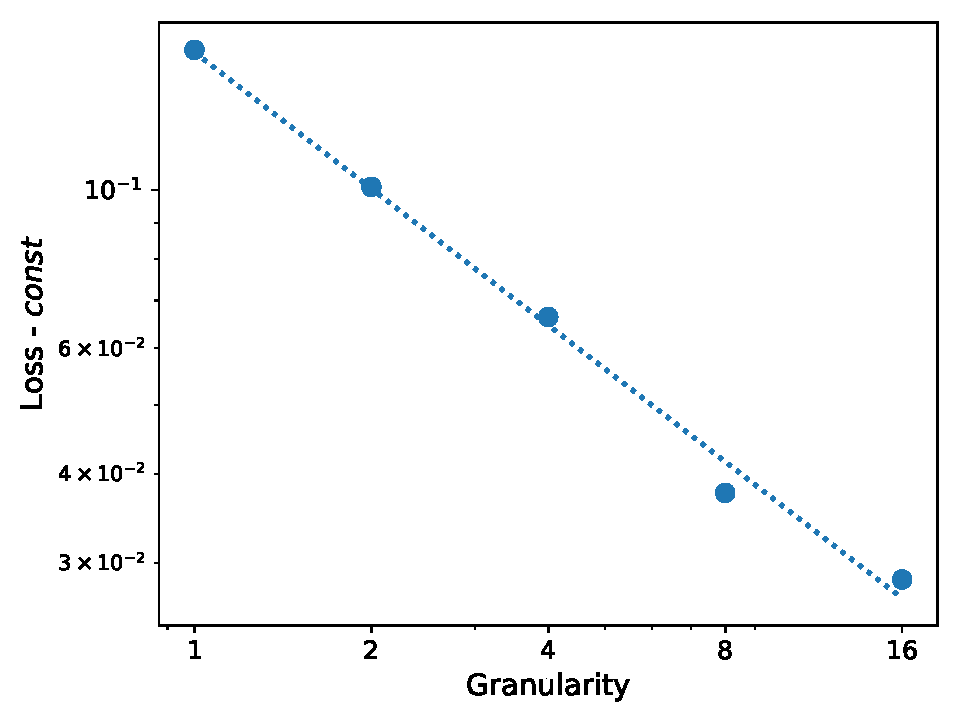
\includegraphics[width=.3\textwidth]{figures/granularity_N_1082130432_D_62500.0.pdf} &
      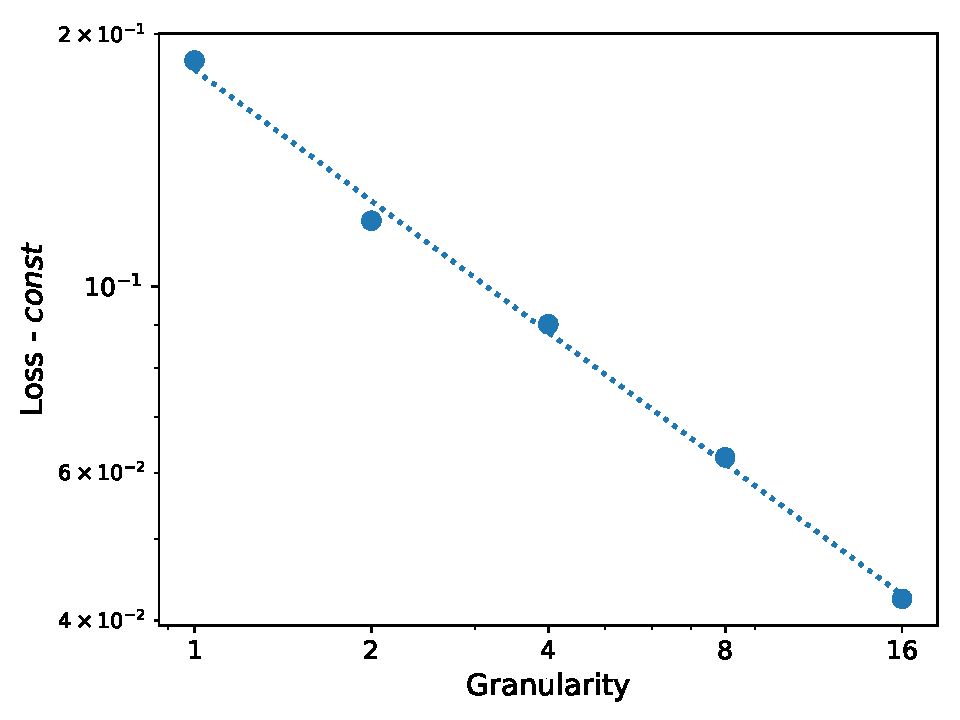
\includegraphics[width=.3\textwidth]{figures/granularity_N_2113536000_D_62500.0.pdf} \\
    \small \textbf{(c)} &
      \small \textbf{(d)}
  \end{tabular}

  \medskip

  \caption{Illustration of scaling granularity when $N, D$ are fixed for: \textbf{(a)} $N=64 \times 25M$, $D=16B$, $const=3.12$ \textbf{(b)} $N=64 \times 49M $, $D=16B$, $const=3.02$ \textbf{(c)} $N=64 \times 25M$,  $D=32B$, $const=3.03$ \textbf{(d)} $N=64 \times 49M$, $D=32B$, $const=2.88$ }
  \label{line_gran_plot_fixed}
\end{figure}
\end{document}
